\section{Some Python Results}


\begin{table}
\centering
\caption{Python subjects}
\label{tab:subjects}
{\scriptsize
\begin{tabular}{l|ll}
%\hline
SUT & LOC & Source \\
\hline
AVL & 225 & TSTL example \cite{avltree} \\
%Hypothesis Heaps & 56 & Hypothesis example \cite{hypheaps} \\
bidict & 569 & \url{http://pythonhosted.org/bidict/home.html} \\
CParser & 5033 & \url{https://github.com/albertz/PyCParser}\\
redis-py & 2722 & \url{https://github.com/andymccurdy/redis-py}\\
python-rsa & 1597 & \url{https://github.com/sybrenstuvel/python-rsa} \\
simplejson & 2811 & \url{https://simplejson.readthedocs.io/en/latest/} \\
sortedcontainers & 2017 & \url{http://www.grantjenks.com/docs/sortedcontainers/} \\
SymPy & 227959 & \url{http://www.sympy.org/en/index.html} \\
%\hline
\end{tabular}
}
\end{table}

Table \ref{tab:subjects} describes the Python subjects, tested using
the TSTL \cite{tstlsttt,NFM15} harnesses included in the TSTL
distribution.  Of the eight subjects, one is a toy container class
with an injected realistic fault, and the other seven are real-world
Python libraries, with a large number of GitHub stars or high
ranking in pip.  Results are shown for both standard random testing
and swarm testing \cite{ISSTA12}, using 120 seconds of test time.
While the change to swarm testing sometimes changes the effectiveness
curve, shapes at 30 seconds and 60 seconds are very similar, despite
changes in overall coverage obtained.

\newpage

\begin{figure}
%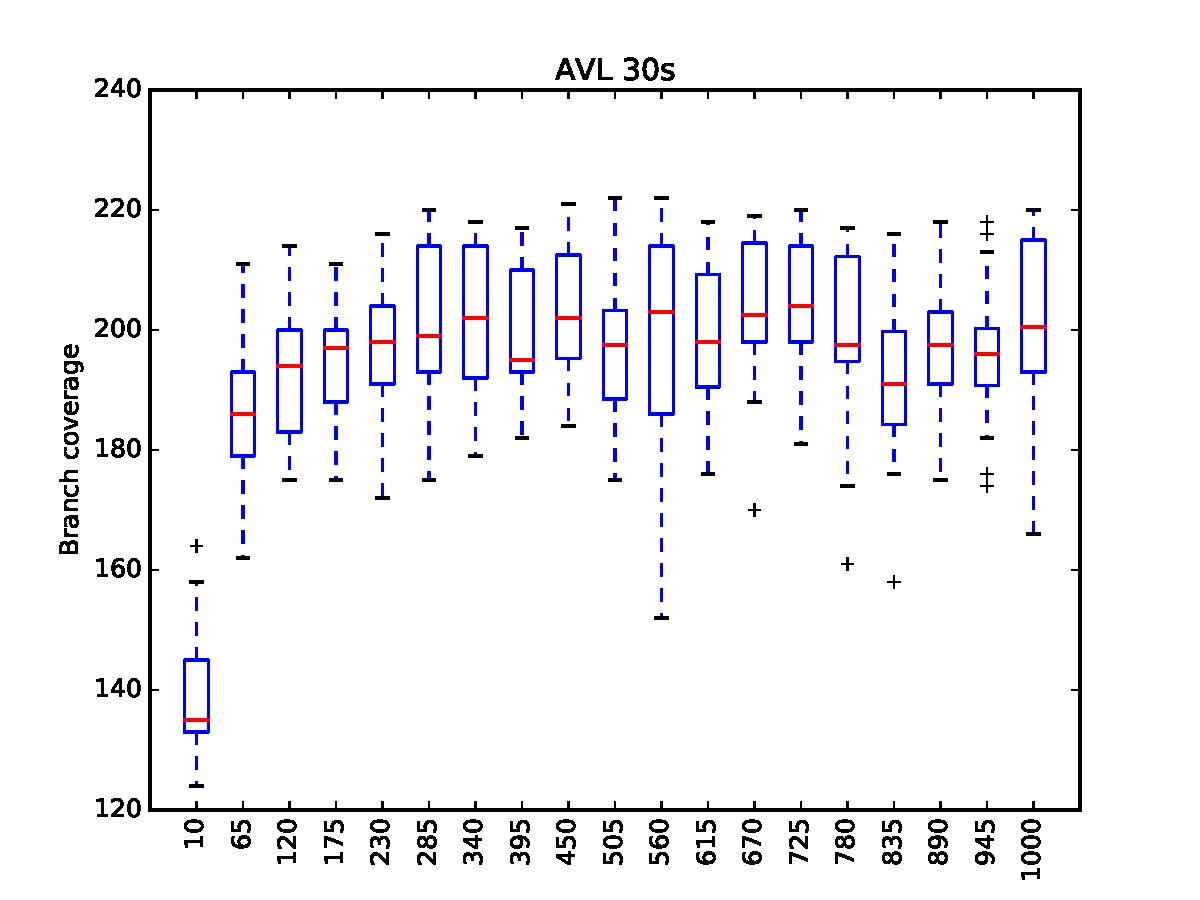
\includegraphics[width=\columnwidth]{graphs/AVLrand30}
%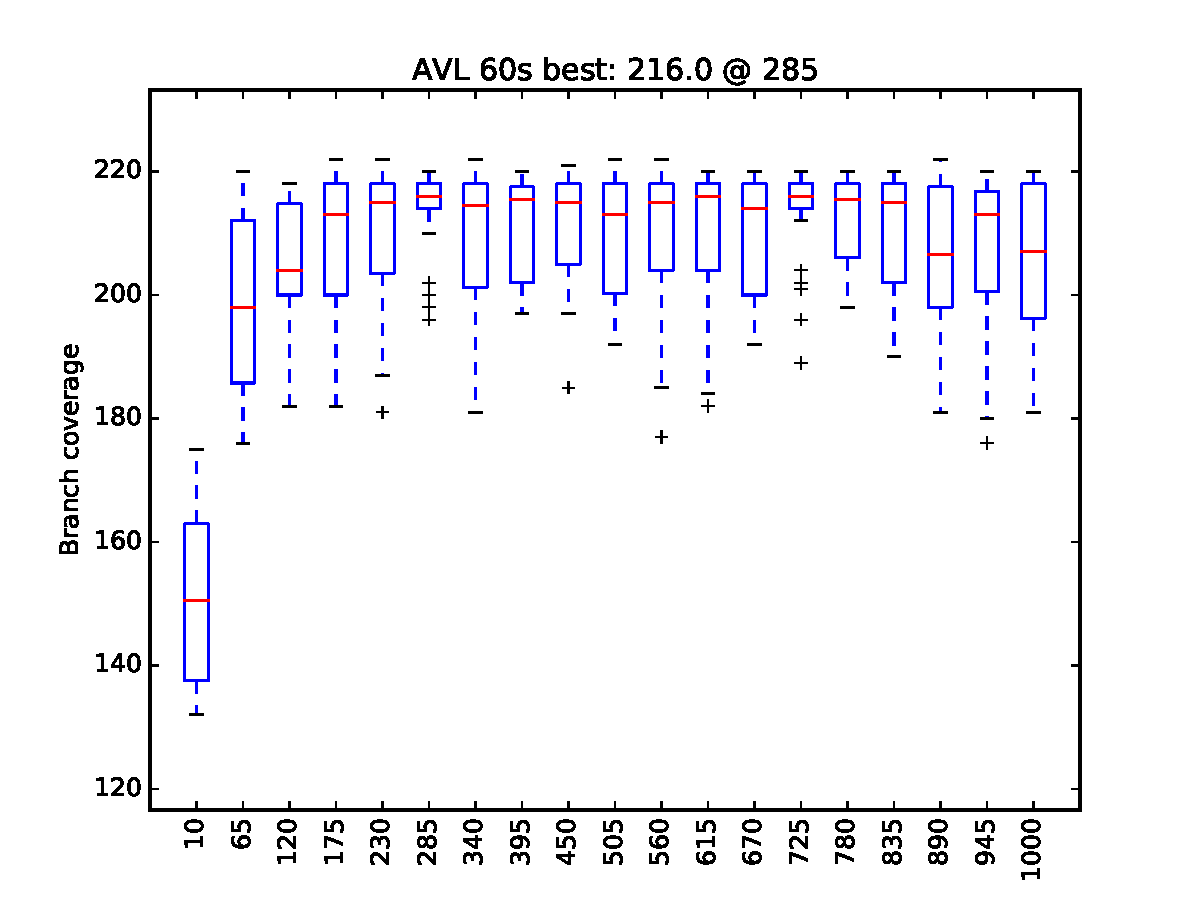
\includegraphics[width=\columnwidth]{graphs/AVLrand60}
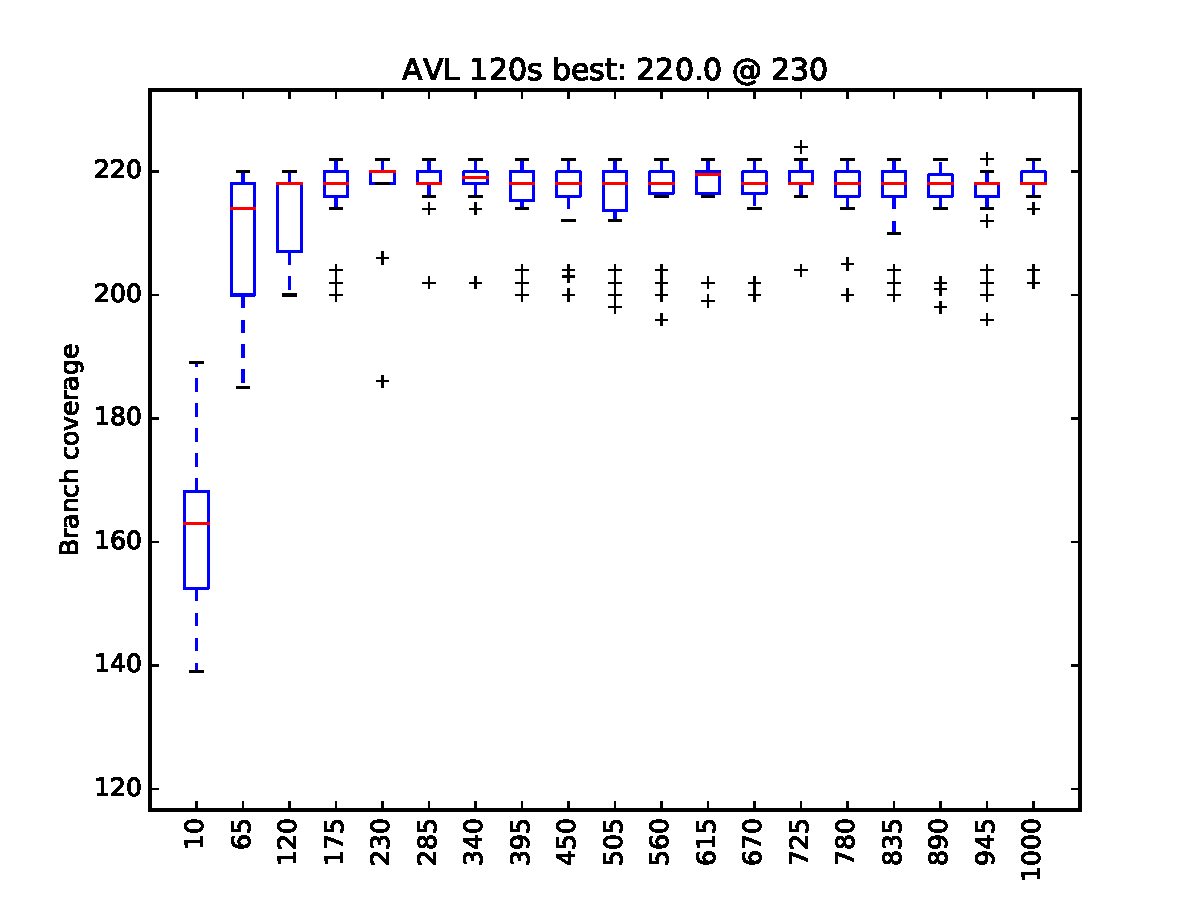
\includegraphics[width=\columnwidth]{graphs/AVLrand120}
\includegraphics[width=\columnwidth]{graphs/opsavlrand120}
\includegraphics[width=\columnwidth]{graphs/execavlrand120}
\end{figure}


\begin{figure}
%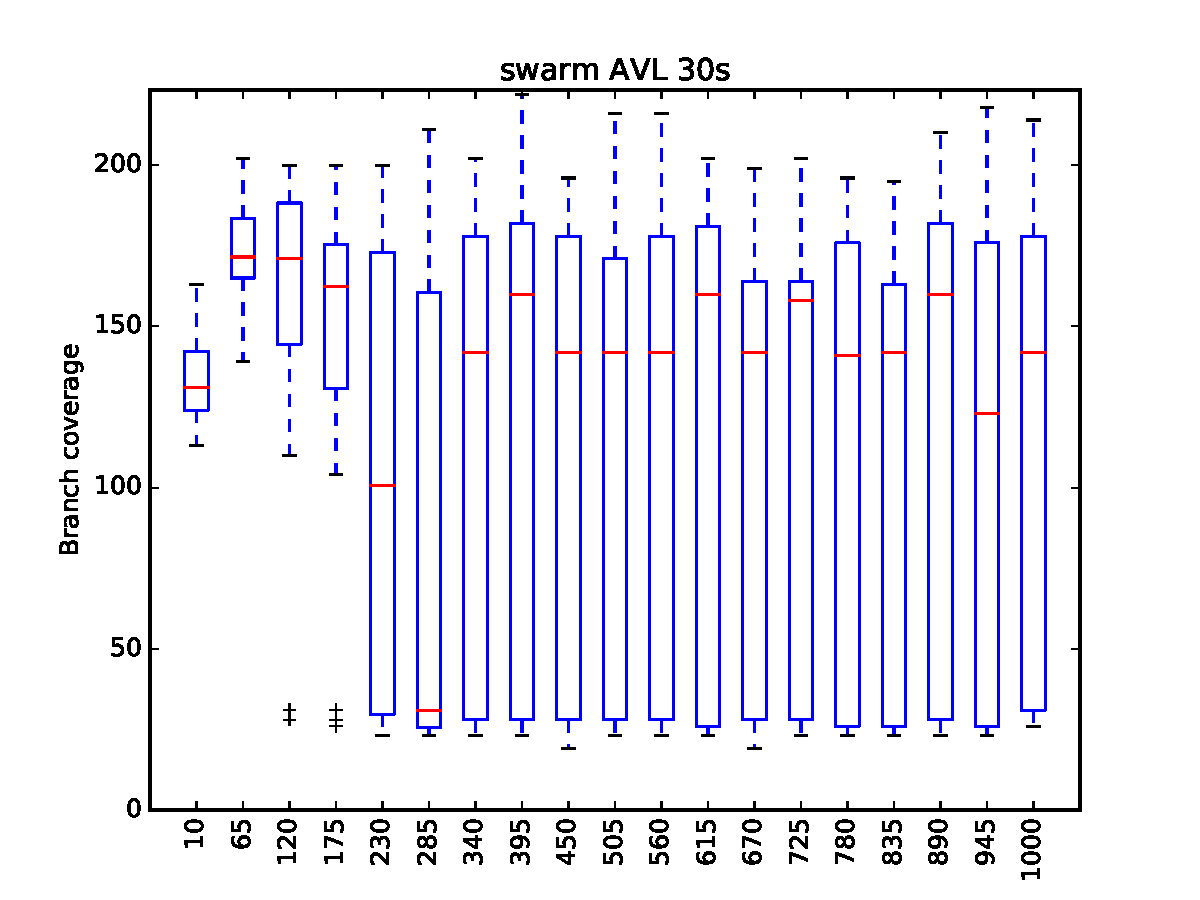
\includegraphics[width=\columnwidth]{graphs/AVLswarm30}
%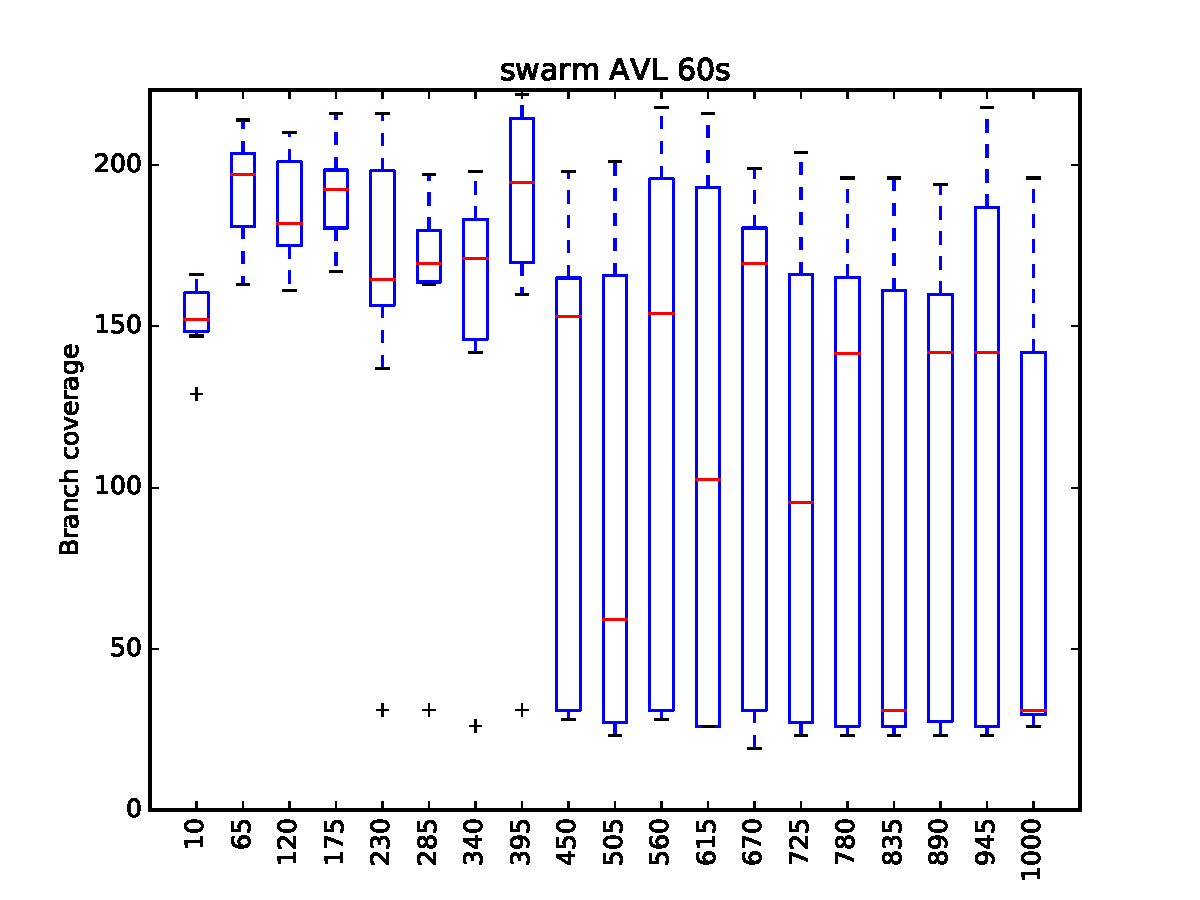
\includegraphics[width=\columnwidth]{graphs/AVLswarm60}
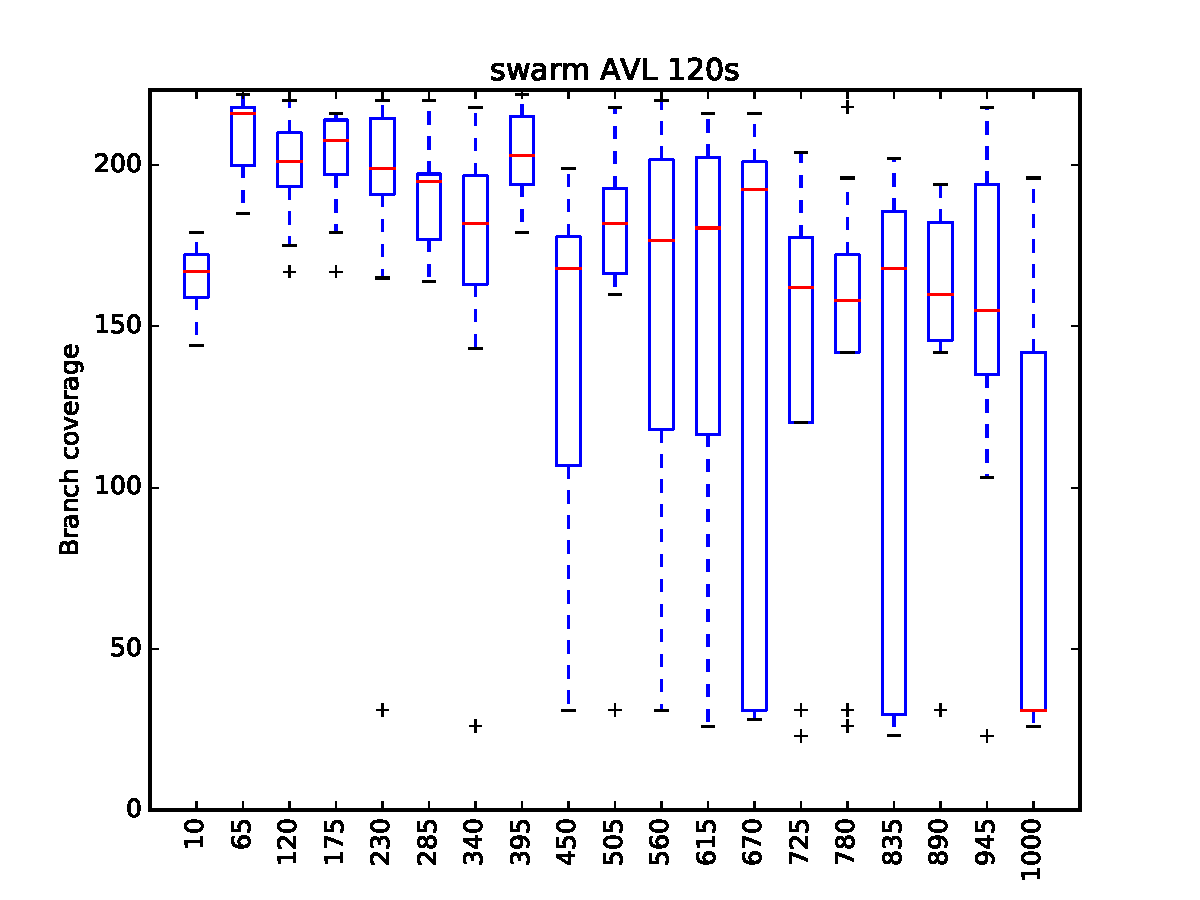
\includegraphics[width=\columnwidth]{graphs/AVLswarm120}
\includegraphics[width=\columnwidth]{graphs/opsavlswarm120}
\includegraphics[width=\columnwidth]{graphs/execavlswarm120}
\end{figure}

\begin{figure}
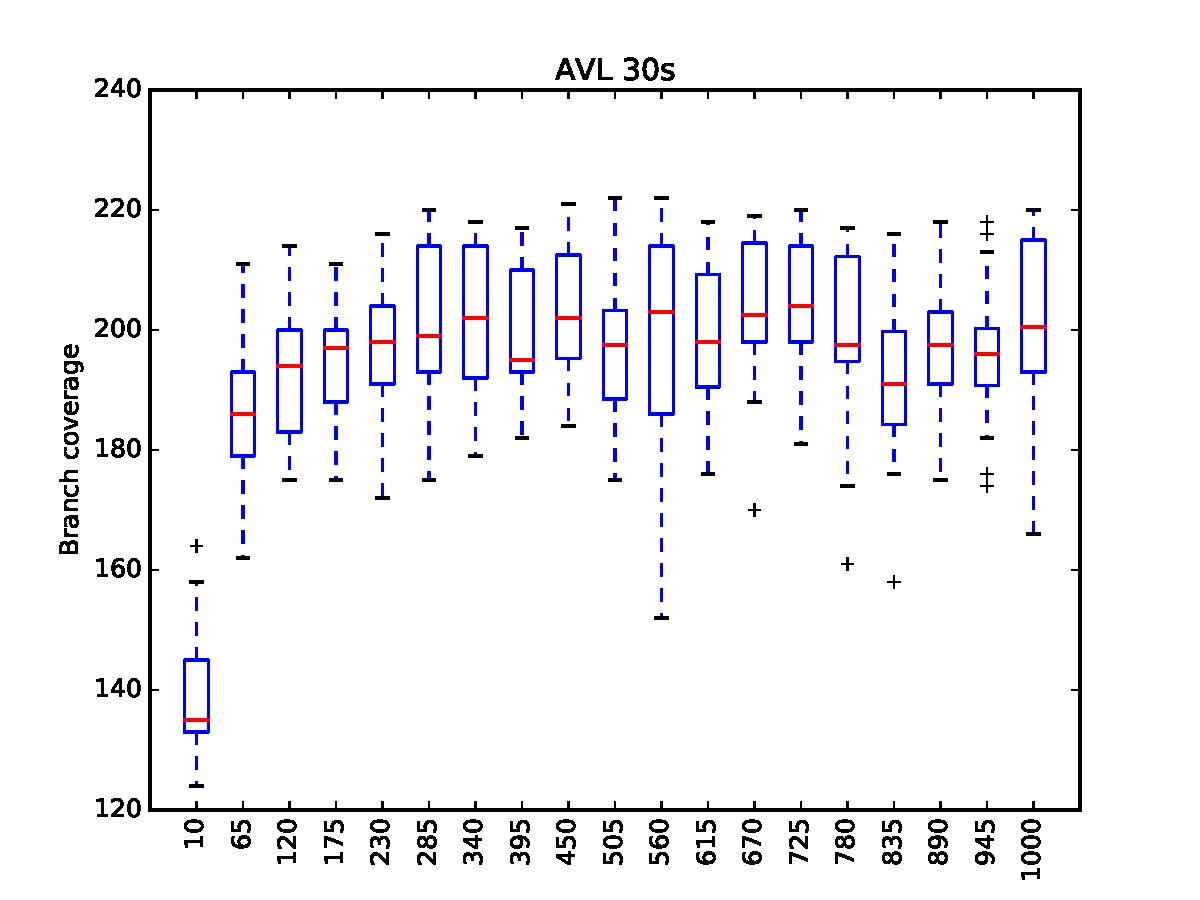
\includegraphics[width=\columnwidth]{graphs/AVLrand30}
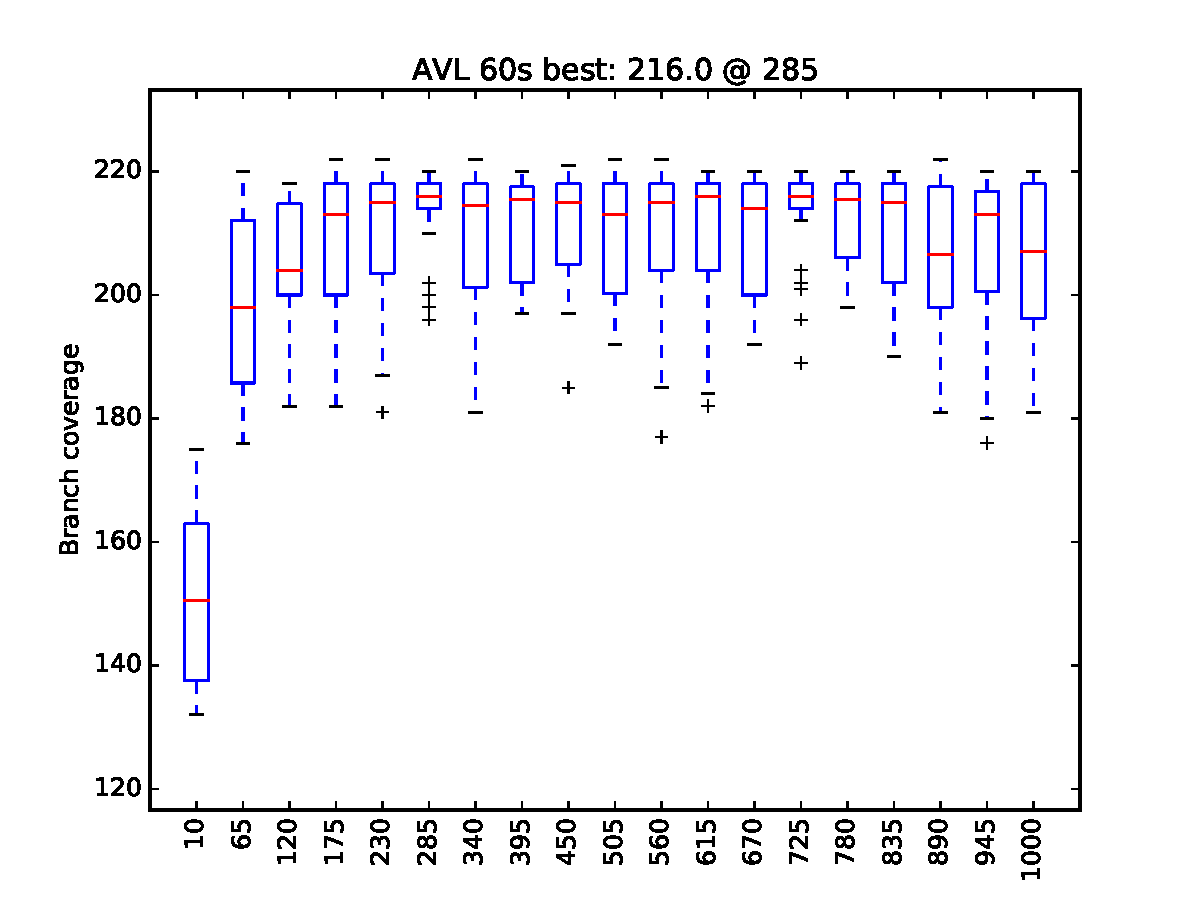
\includegraphics[width=\columnwidth]{graphs/AVLrand60}
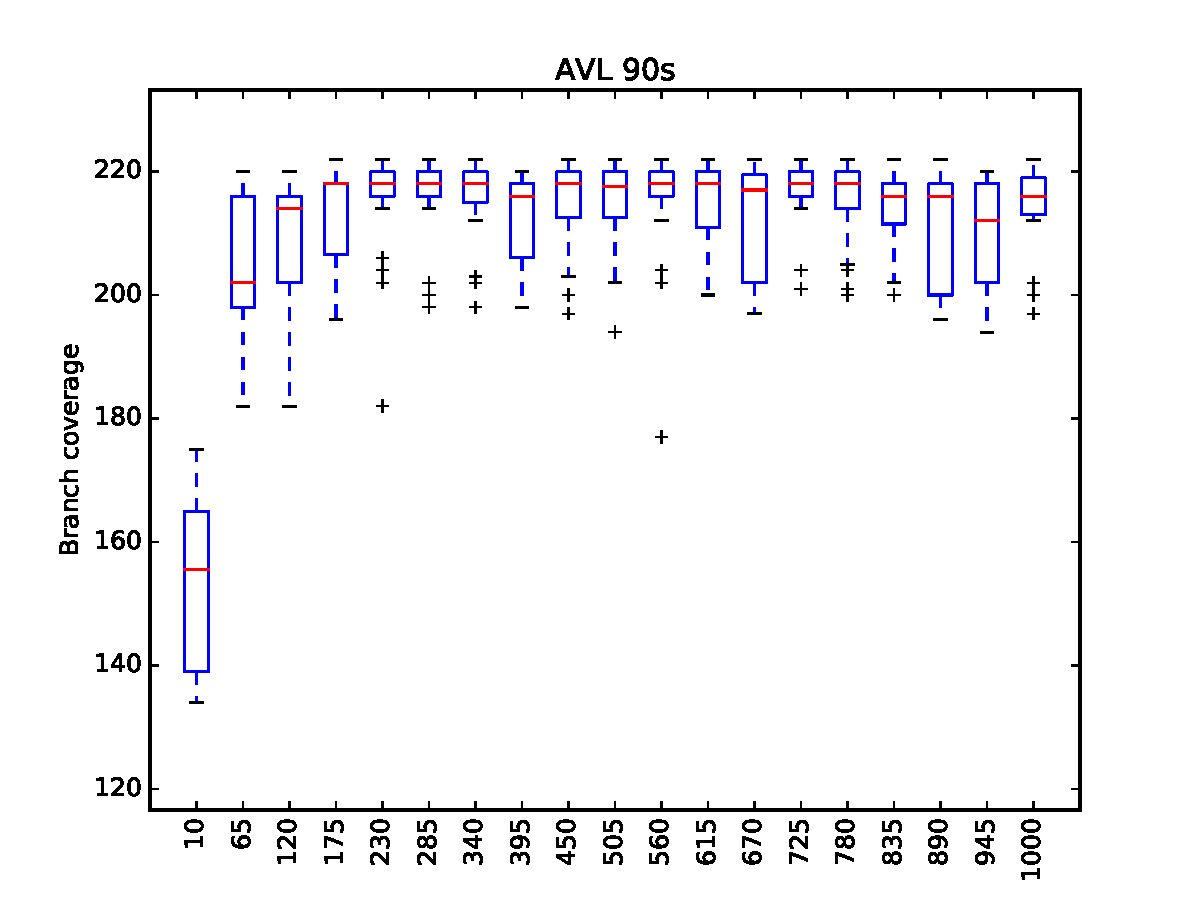
\includegraphics[width=\columnwidth]{graphs/AVLrand90}
%\includegraphics[width=\columnwidth]{graphs/opsavlrand120}
%\includegraphics[width=\columnwidth]{graphs/execavlrand120}
\end{figure}

\begin{figure}
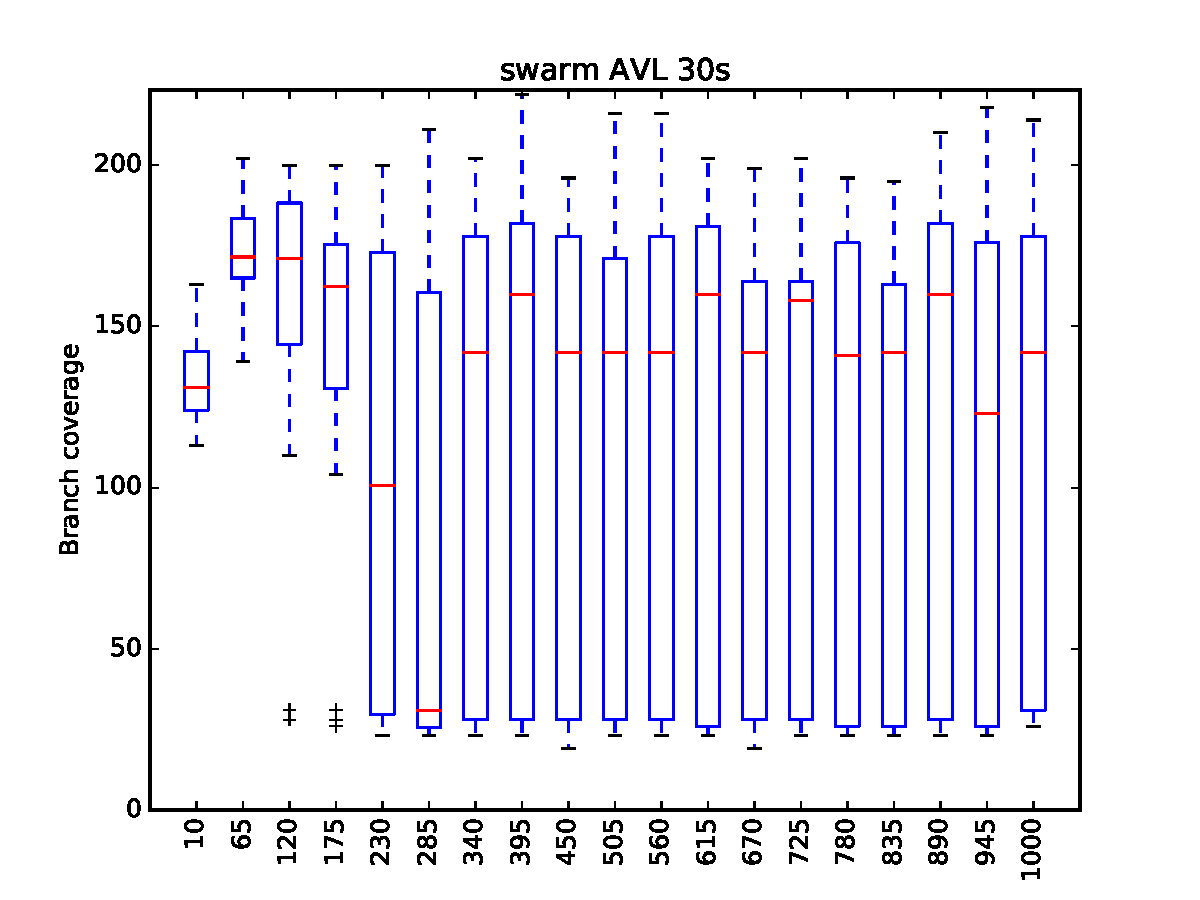
\includegraphics[width=\columnwidth]{graphs/AVLswarm30}
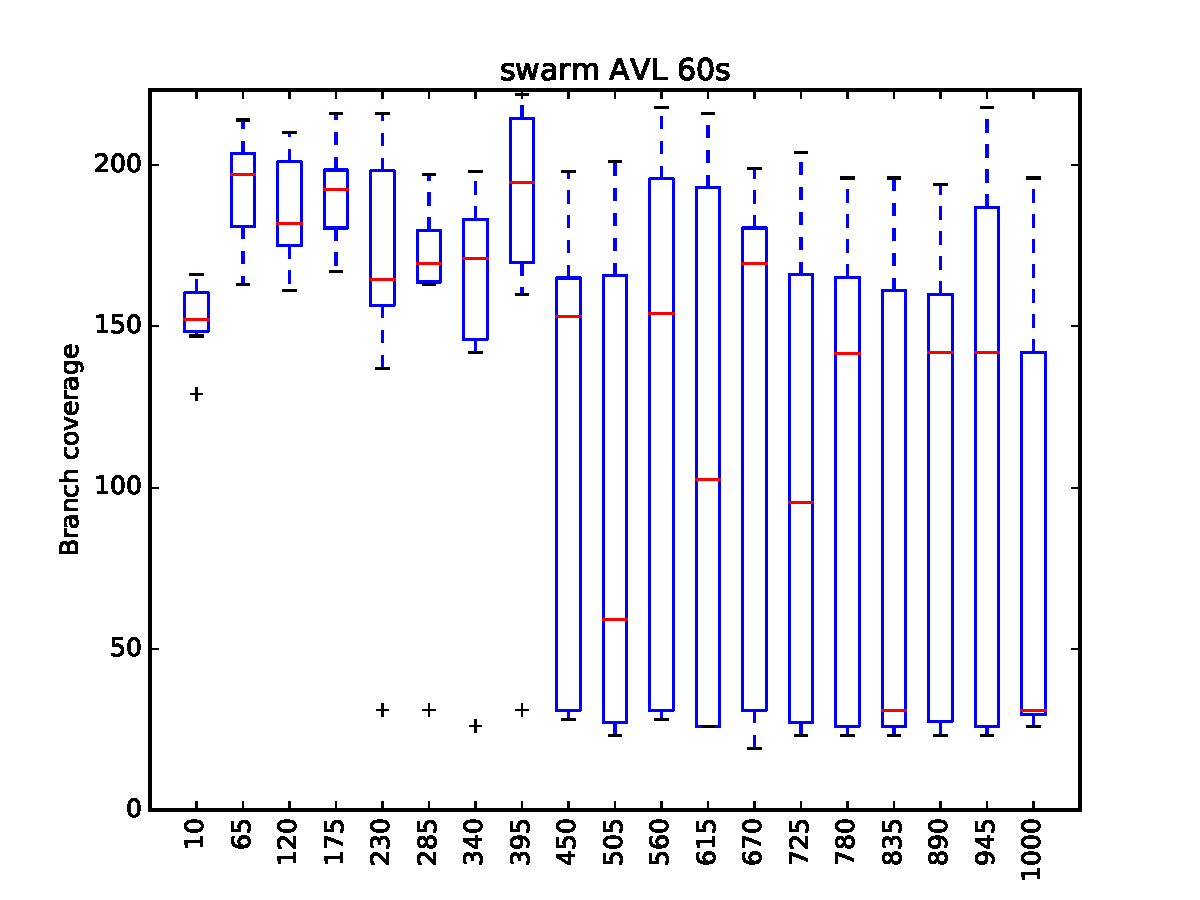
\includegraphics[width=\columnwidth]{graphs/AVLswarm60}
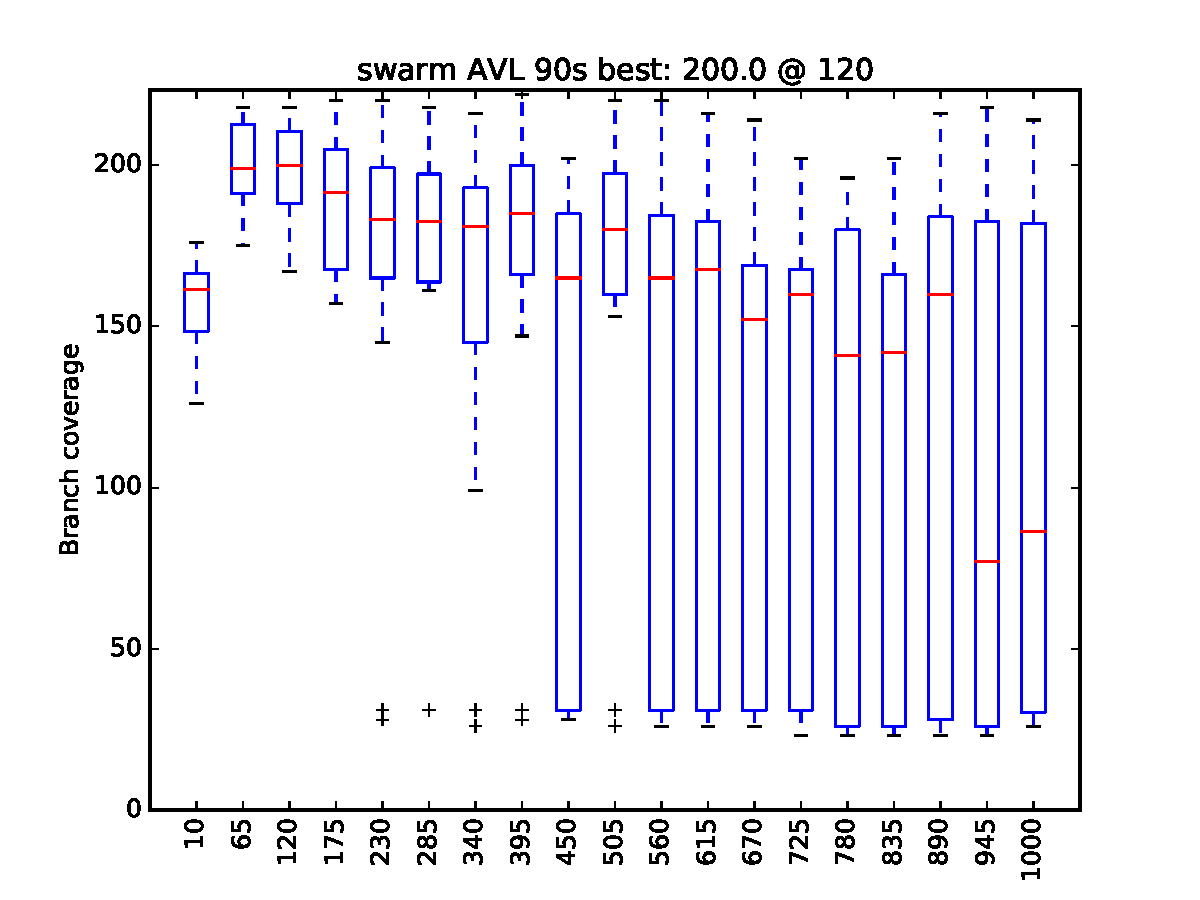
\includegraphics[width=\columnwidth]{graphs/AVLswarm90}
%\includegraphics[width=\columnwidth]{graphs/opsavlrand120}
%\includegraphics[width=\columnwidth]{graphs/execavlrand120}
\end{figure}

\begin{figure}
%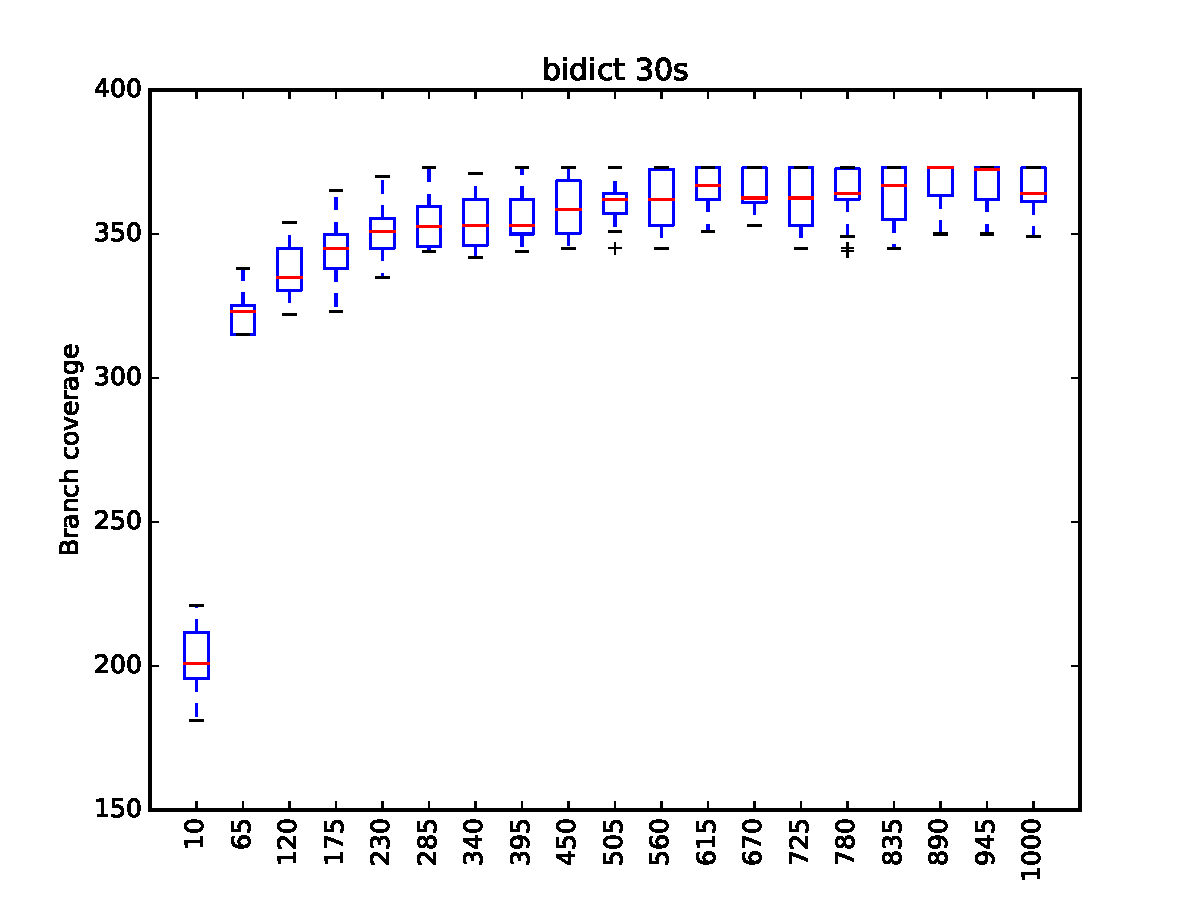
\includegraphics[width=\columnwidth]{graphs/bidictrand30}
%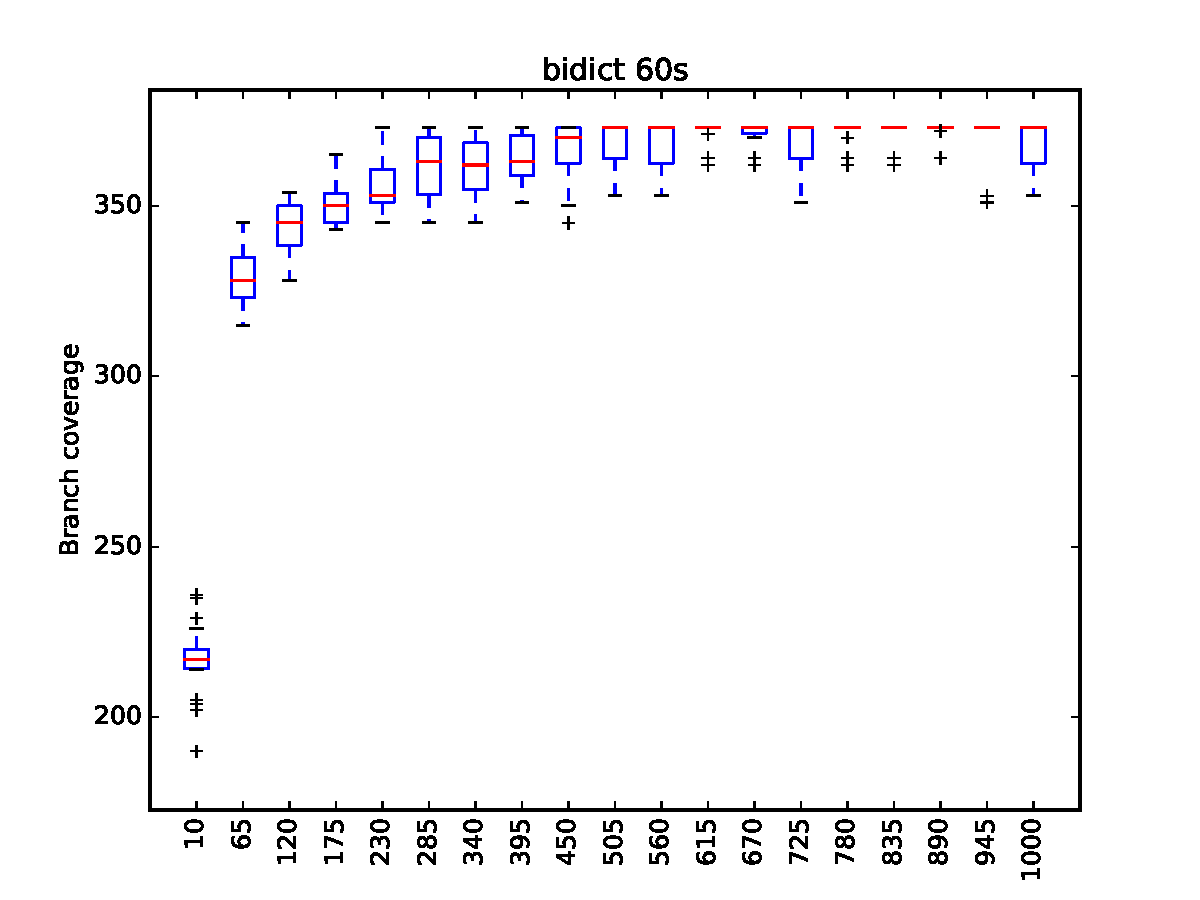
\includegraphics[width=\columnwidth]{graphs/bidictrand60}
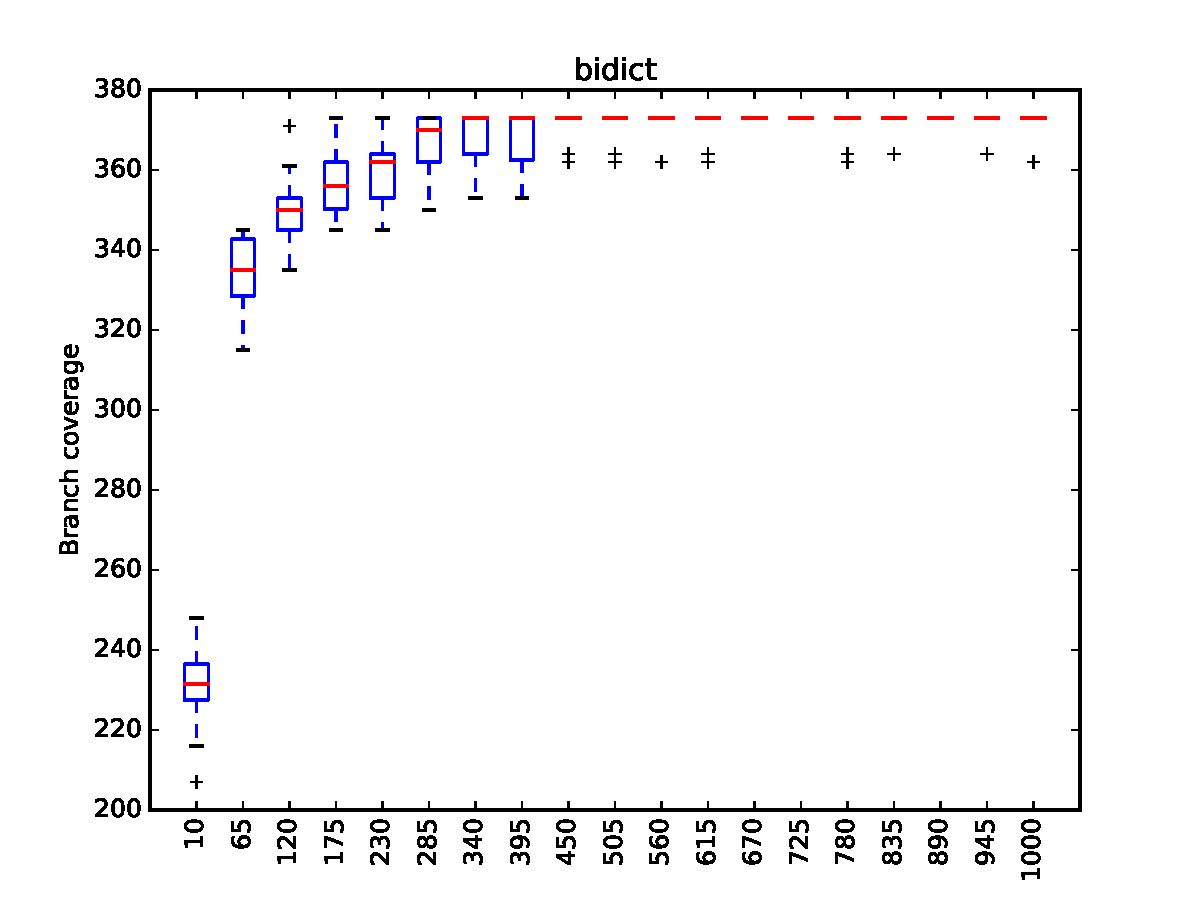
\includegraphics[width=\columnwidth]{graphs/bidictrand120}
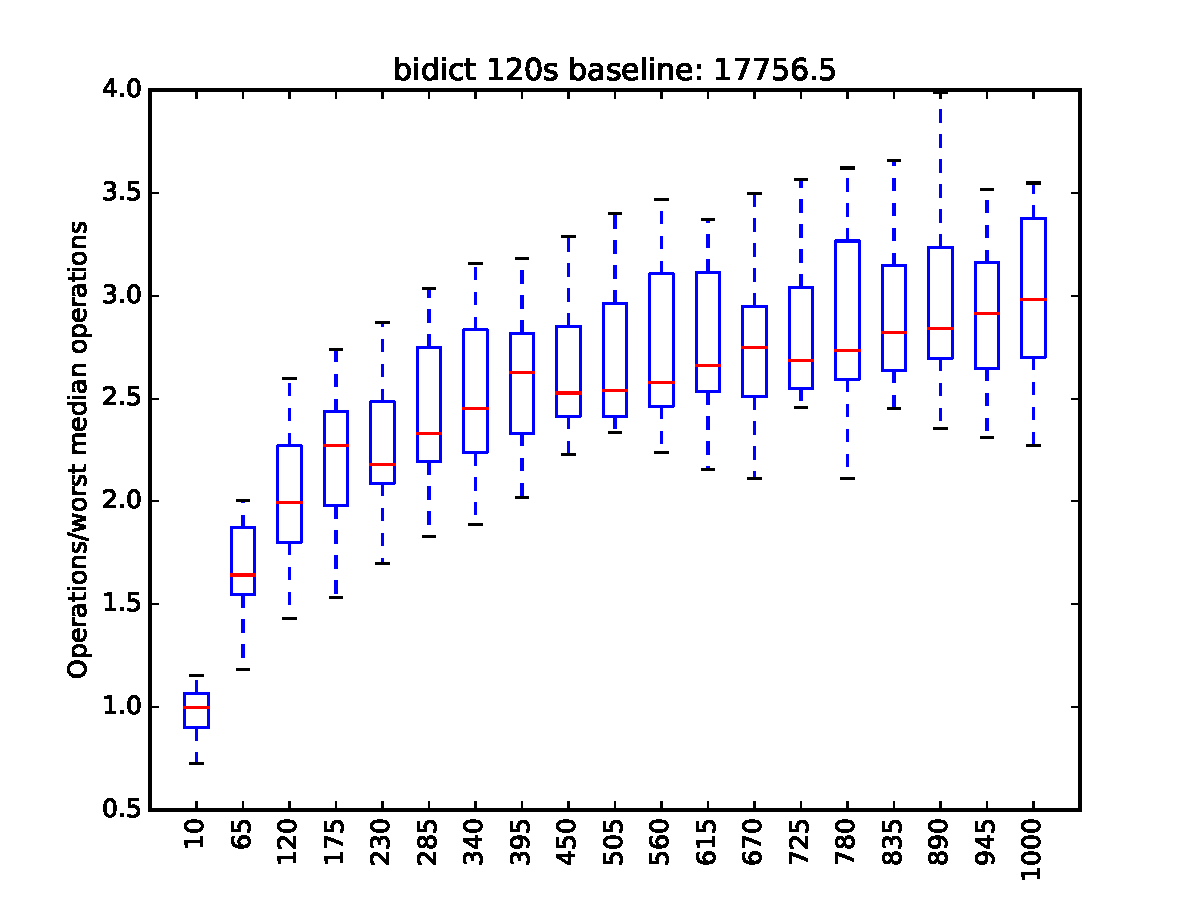
\includegraphics[width=\columnwidth]{graphs/opsbidictrand120}
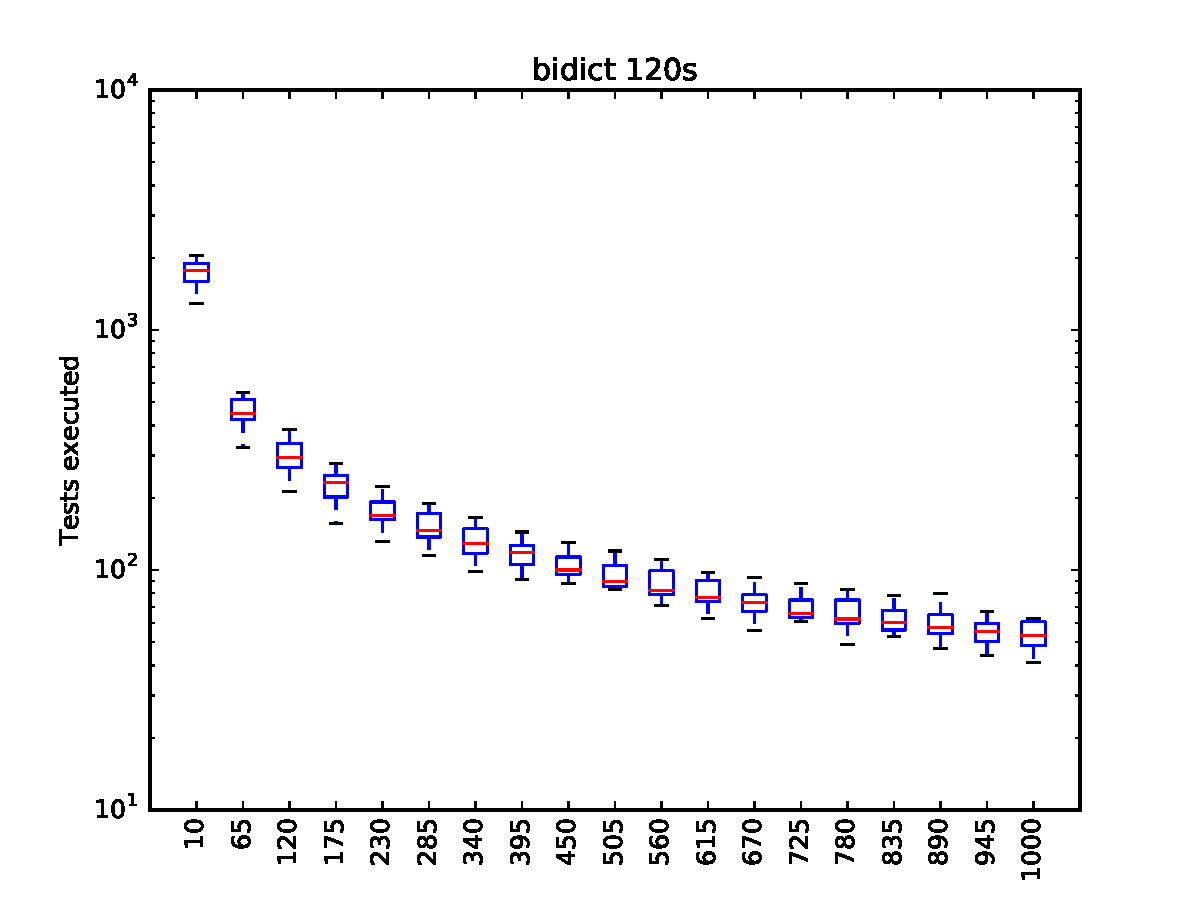
\includegraphics[width=\columnwidth]{graphs/execbidictrand120}
\end{figure}


\begin{figure}
%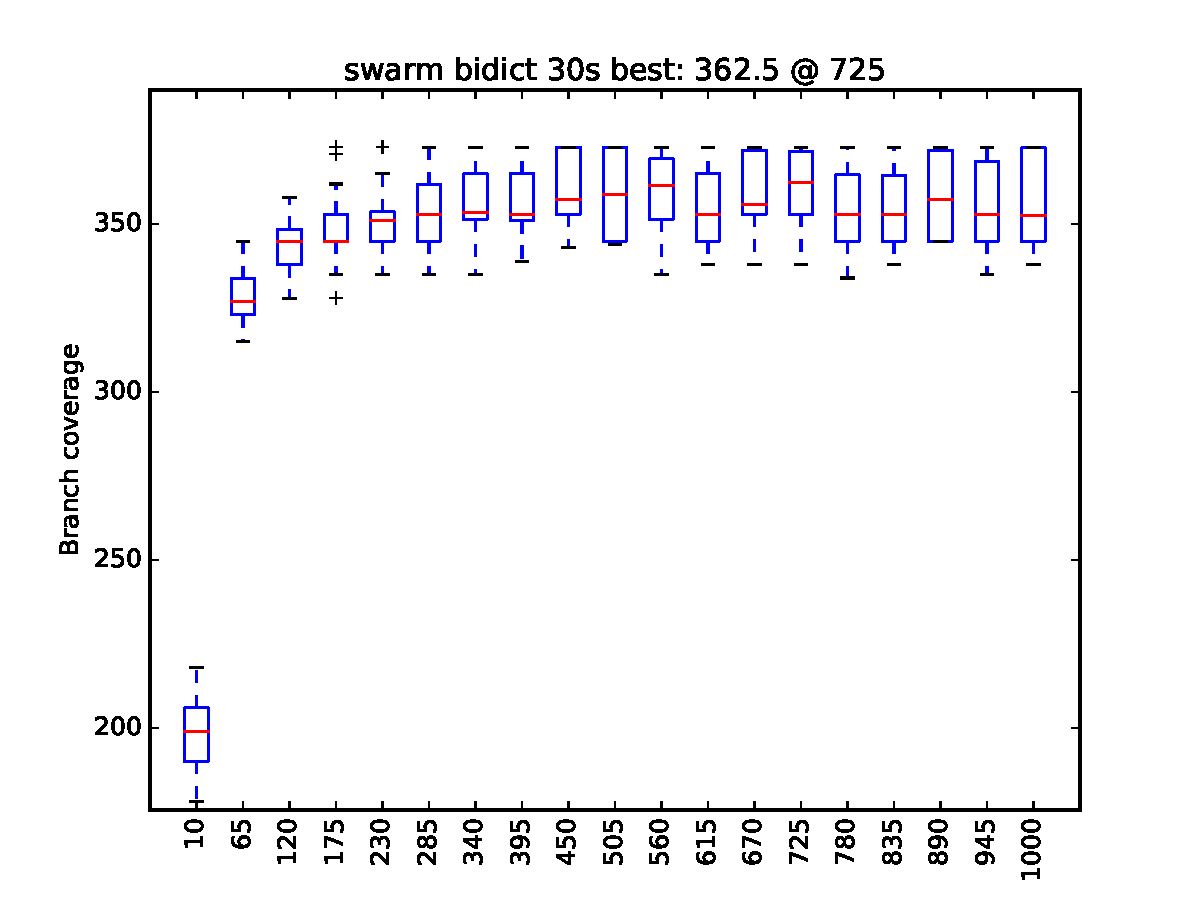
\includegraphics[width=\columnwidth]{graphs/bidictswarm30}
%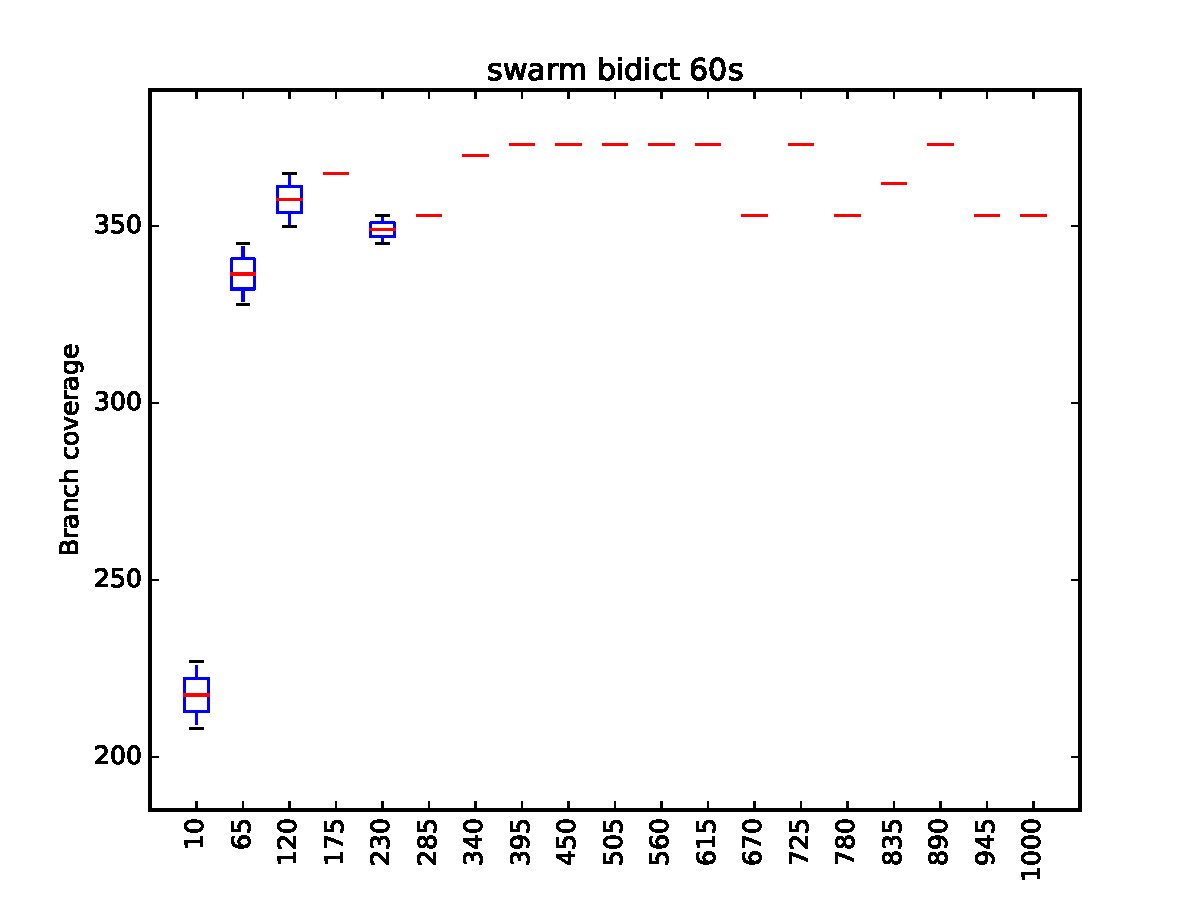
\includegraphics[width=\columnwidth]{graphs/bidictswarm60}
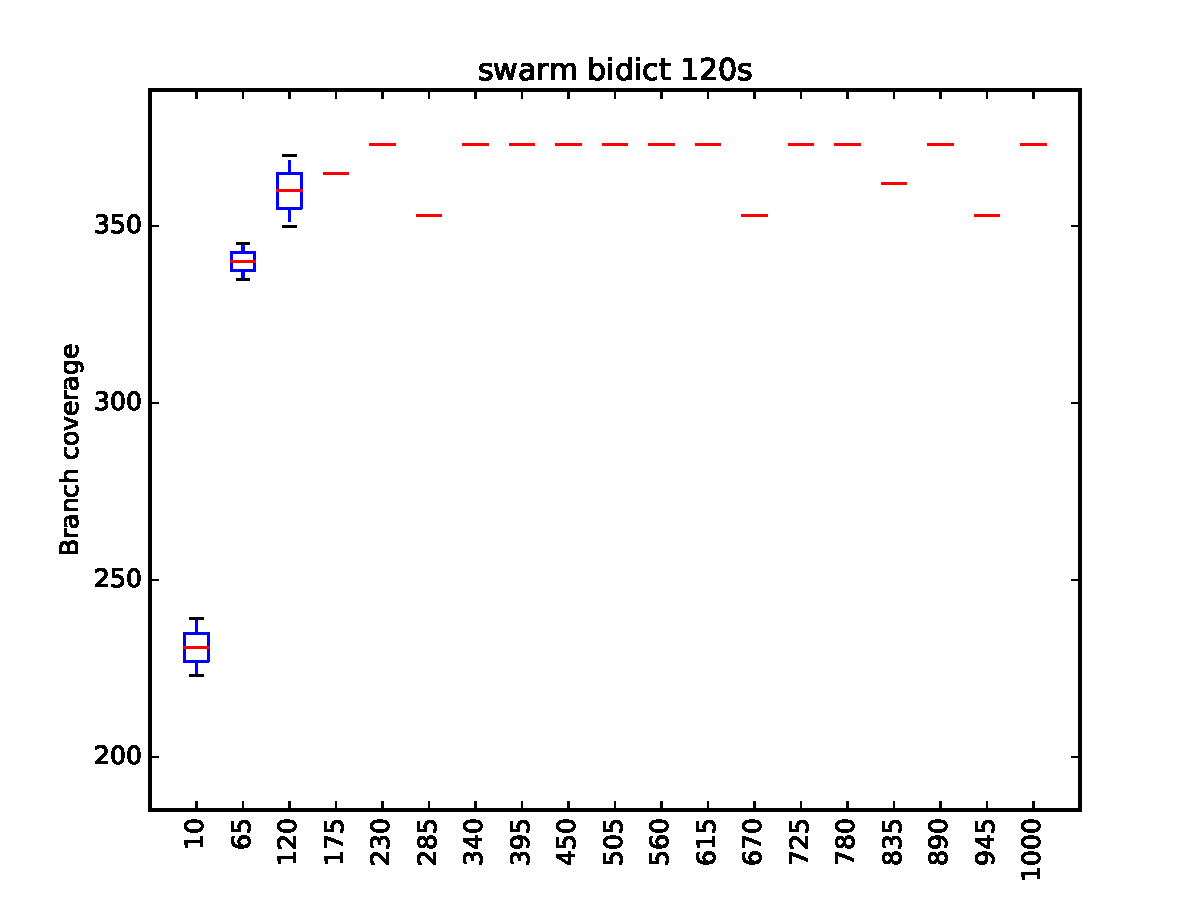
\includegraphics[width=\columnwidth]{graphs/bidictswarm120}
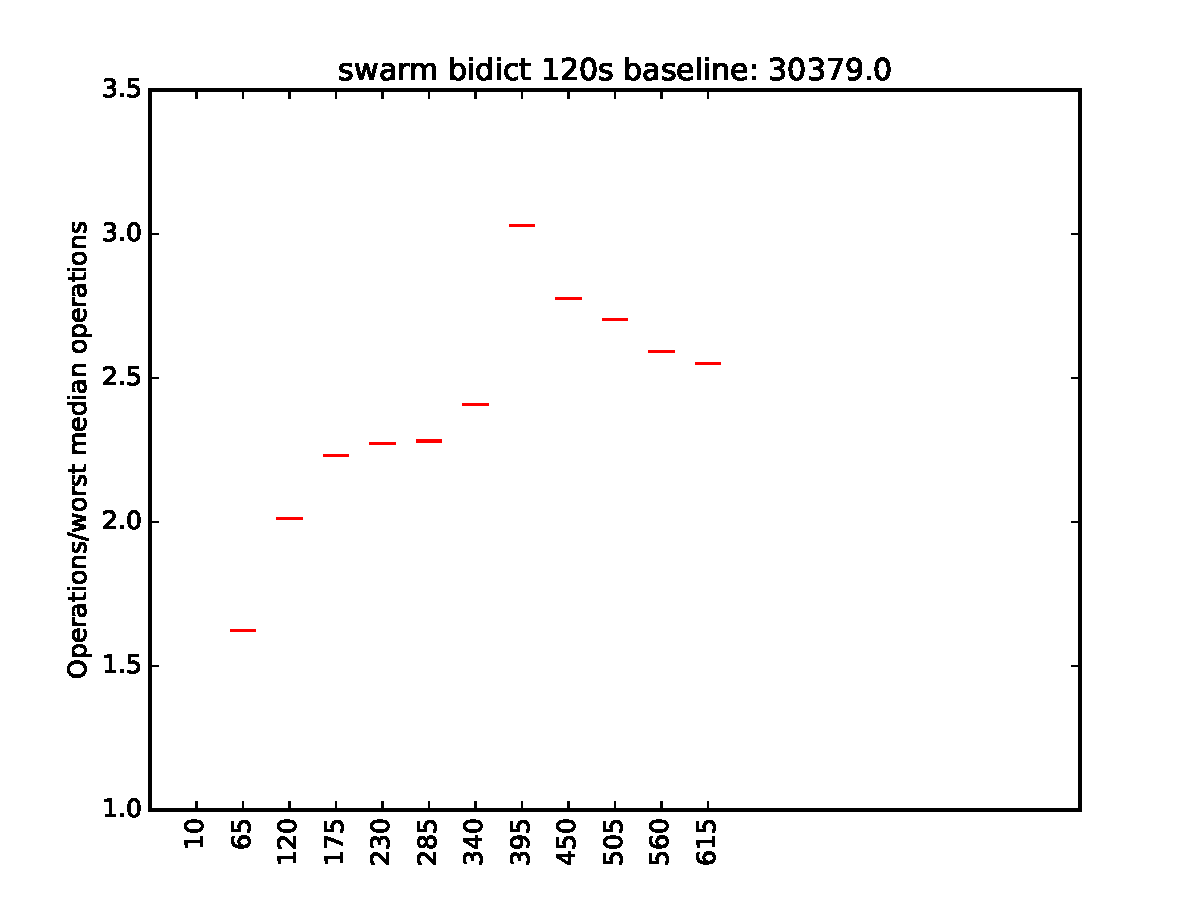
\includegraphics[width=\columnwidth]{graphs/opsbidictswarm120}
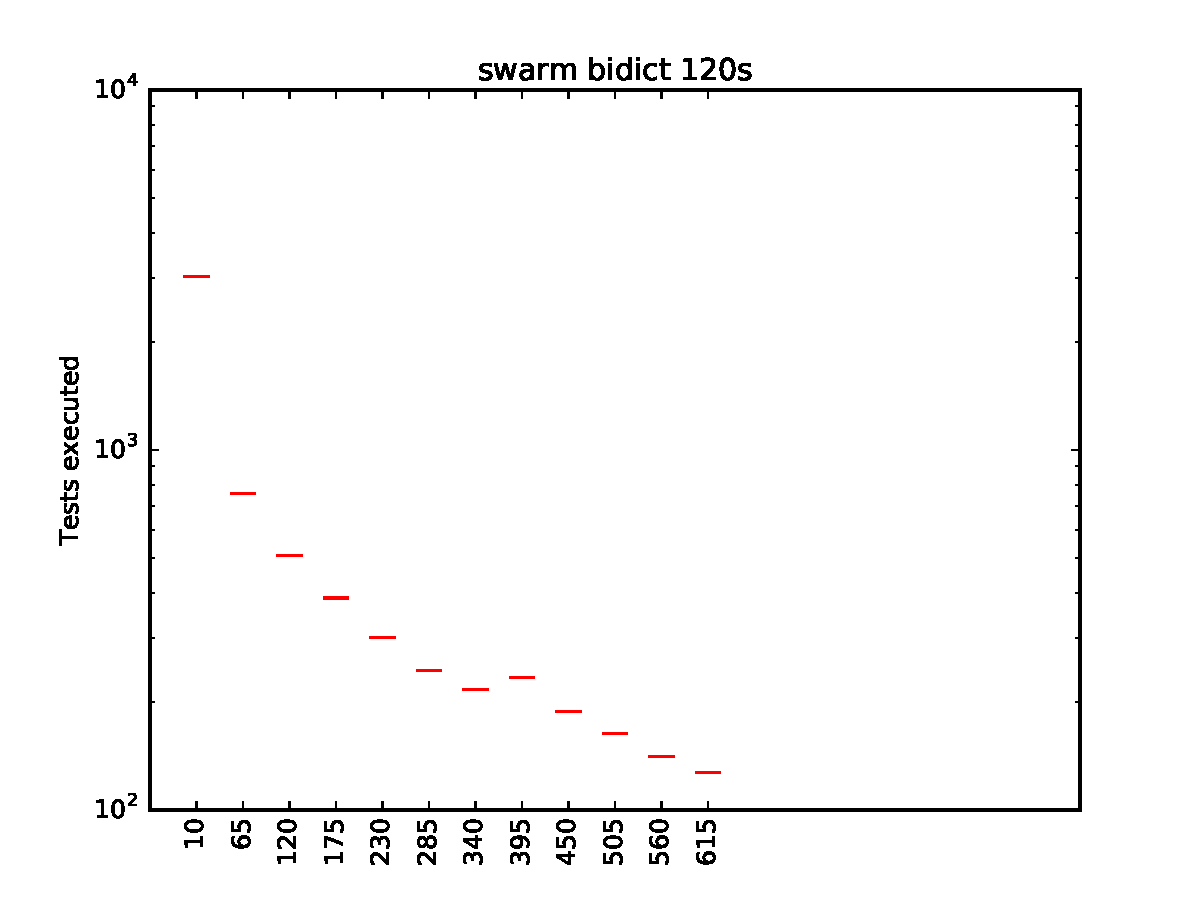
\includegraphics[width=\columnwidth]{graphs/execbidictswarm120}
\end{figure}


\begin{figure}
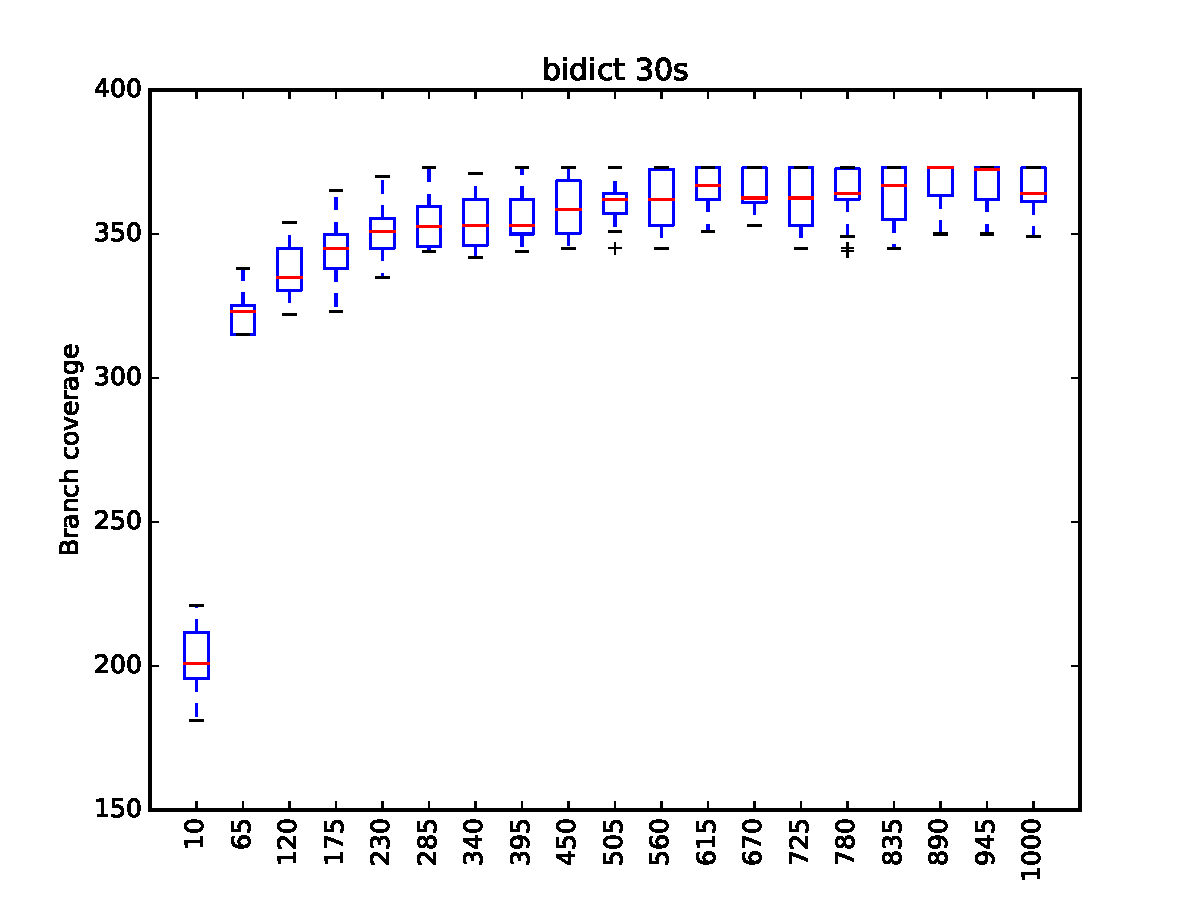
\includegraphics[width=\columnwidth]{graphs/bidictrand30}
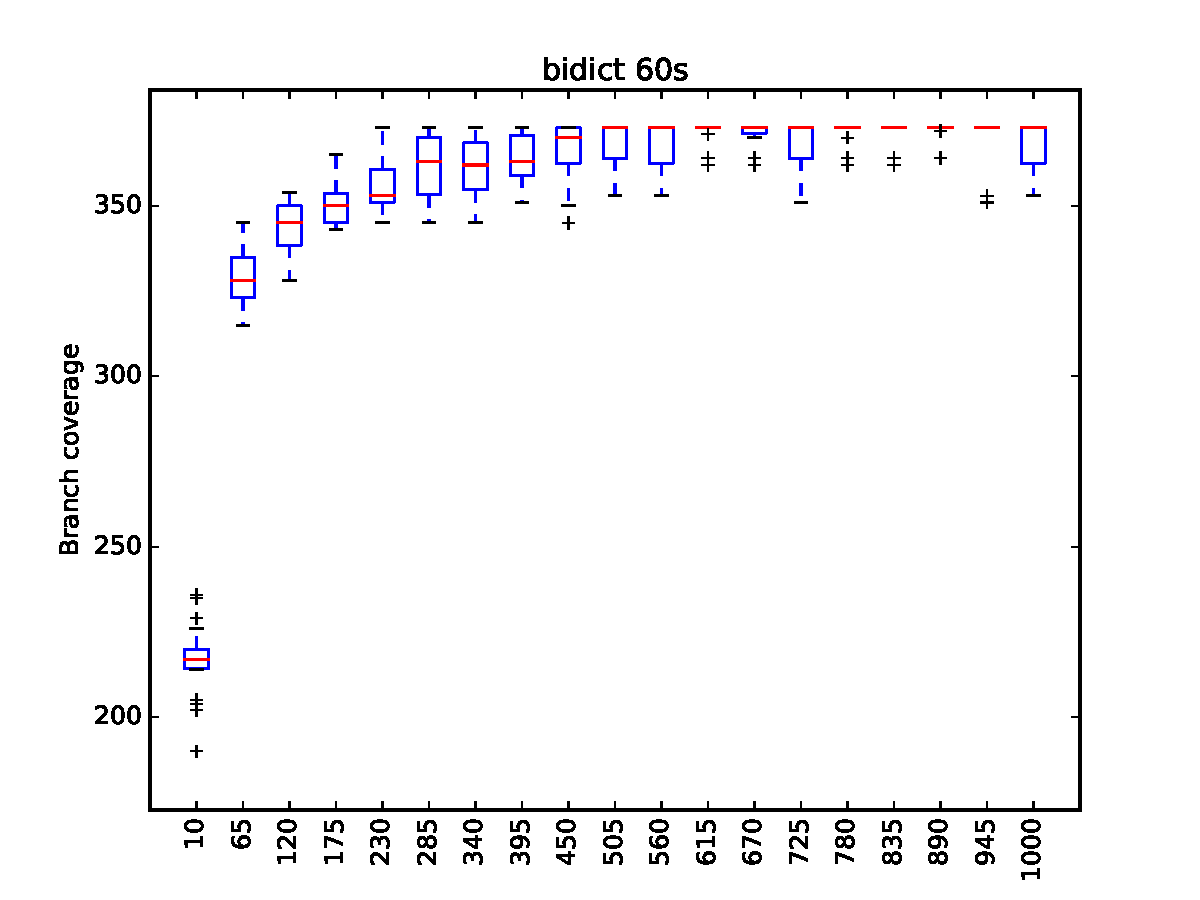
\includegraphics[width=\columnwidth]{graphs/bidictrand60}
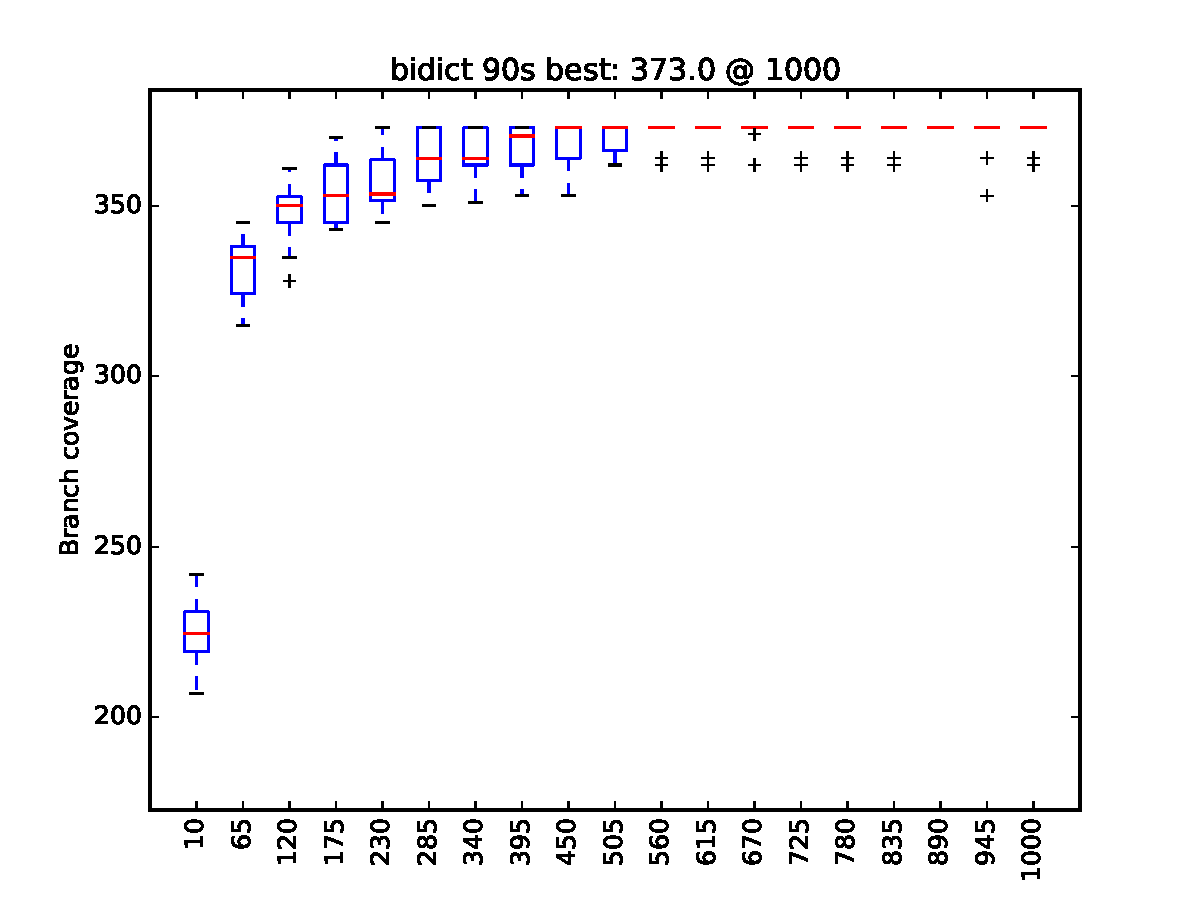
\includegraphics[width=\columnwidth]{graphs/bidictrand90}
%\includegraphics[width=\columnwidth]{graphs/opsavlrand120}
%\includegraphics[width=\columnwidth]{graphs/execavlrand120}
\end{figure}

\begin{figure}
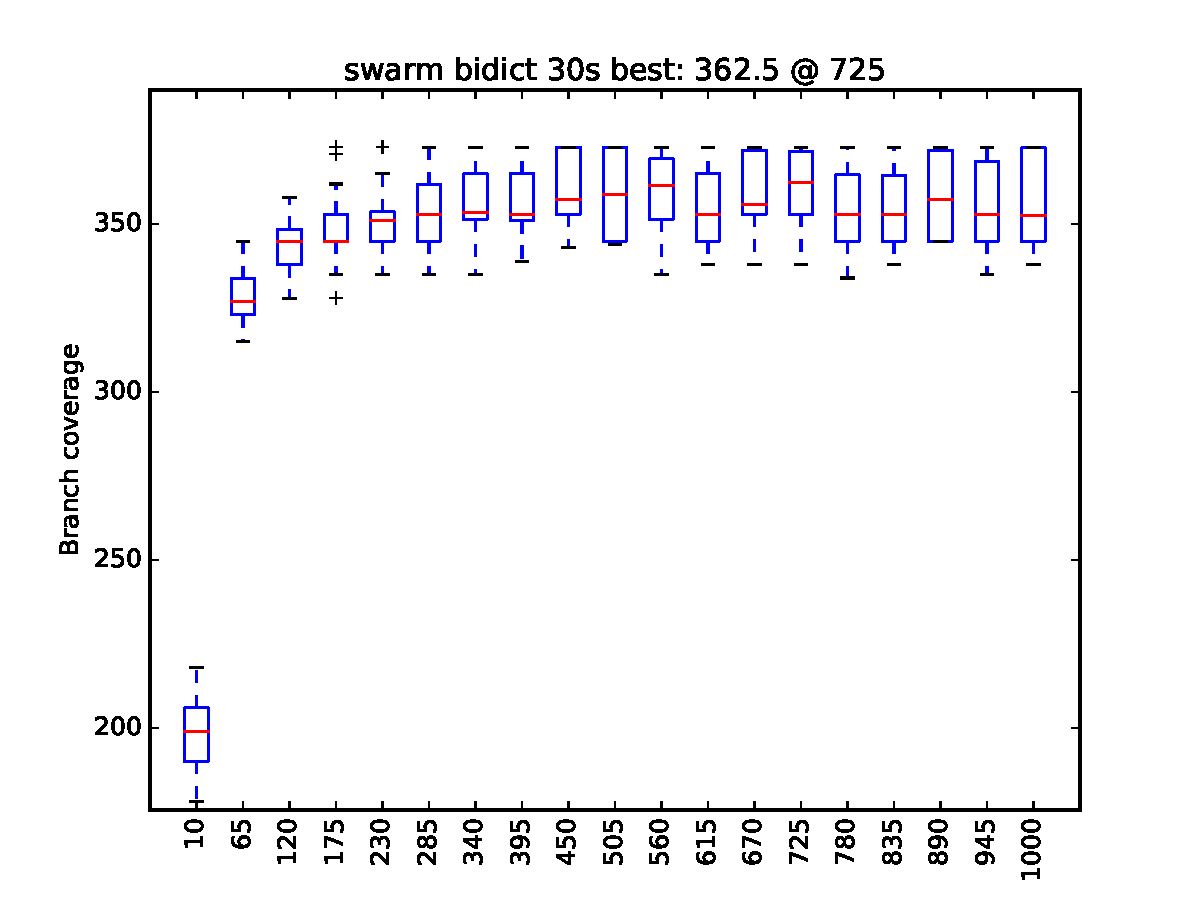
\includegraphics[width=\columnwidth]{graphs/bidictswarm30}
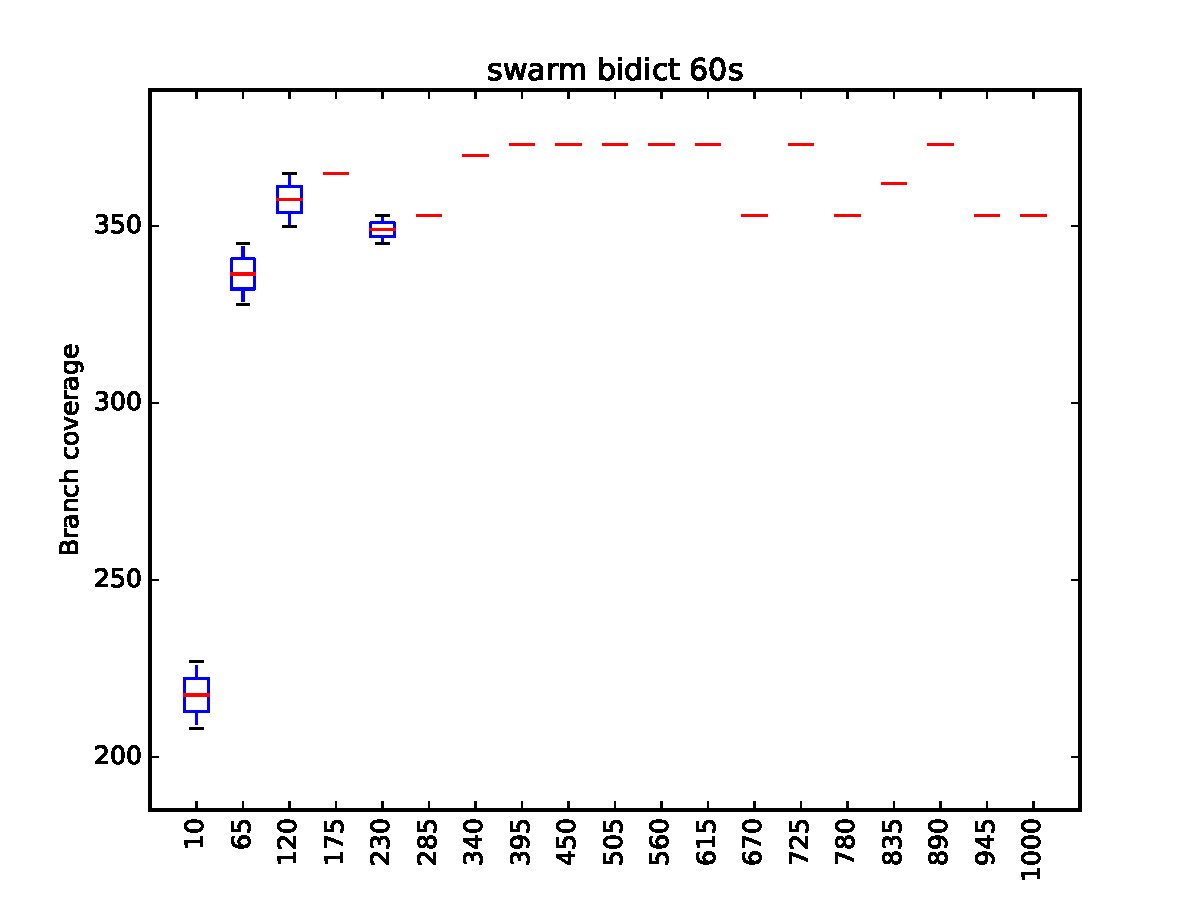
\includegraphics[width=\columnwidth]{graphs/bidictswarm60}
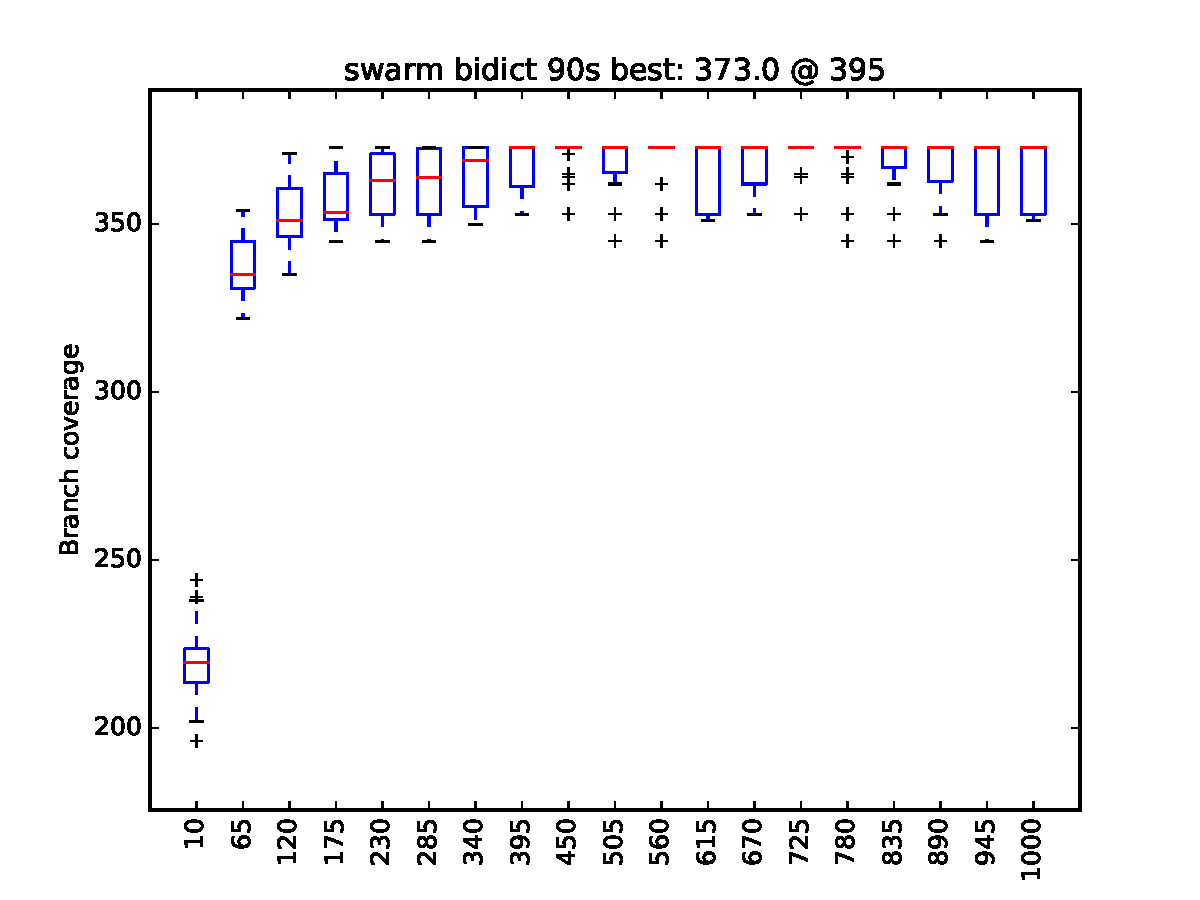
\includegraphics[width=\columnwidth]{graphs/bidictswarm90}
%\includegraphics[width=\columnwidth]{graphs/opsavlrand120}
%\includegraphics[width=\columnwidth]{graphs/execavlrand120}
\end{figure}



\begin{figure}
%\includegraphics[width=\columnwidth]{graphs/Crand30}
%\includegraphics[width=\columnwidth]{graphs/Crand60}
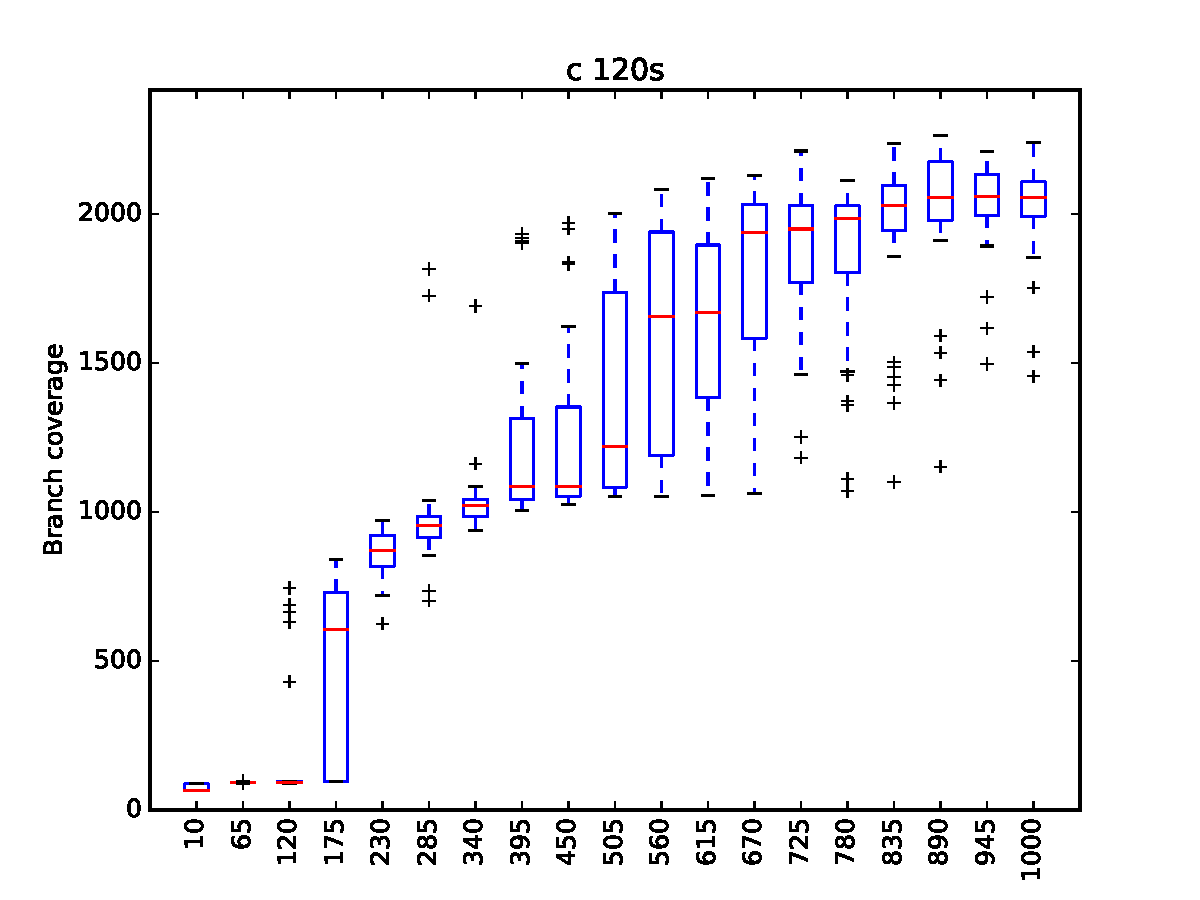
\includegraphics[width=\columnwidth]{graphs/Crand120}
\includegraphics[width=\columnwidth]{graphs/opsCrand120}
\includegraphics[width=\columnwidth]{graphs/execCrand120}
\end{figure}



\begin{figure}
%\includegraphics[width=\columnwidth]{graphs/Cswarm30}
%\includegraphics[width=\columnwidth]{graphs/Cswarm60}
\includegraphics[width=\columnwidth]{graphs/Cswarm120}
\includegraphics[width=\columnwidth]{graphs/opsCswarm120}
\includegraphics[width=\columnwidth]{graphs/execCswarm120}
\end{figure}


\begin{figure}
\includegraphics[width=\columnwidth]{graphs/Crand30}
\includegraphics[width=\columnwidth]{graphs/Crand60}
\includegraphics[width=\columnwidth]{graphs/Crand90}
%\includegraphics[width=\columnwidth]{graphs/opsavlrand120}
%\includegraphics[width=\columnwidth]{graphs/execavlrand120}
\end{figure}

\begin{figure}
\includegraphics[width=\columnwidth]{graphs/Cswarm30}
\includegraphics[width=\columnwidth]{graphs/Cswarm60}
\includegraphics[width=\columnwidth]{graphs/Cswarm90}
%\includegraphics[width=\columnwidth]{graphs/opsavlrand120}
%\includegraphics[width=\columnwidth]{graphs/execavlrand120}
\end{figure}


\begin{figure}
%\includegraphics[width=\columnwidth]{graphs/redisrand30}
%\includegraphics[width=\columnwidth]{graphs/redisrand60}
\includegraphics[width=\columnwidth]{graphs/redisrand120}
\includegraphics[width=\columnwidth]{graphs/opsredisrand120}
\includegraphics[width=\columnwidth]{graphs/execredisrand120}
\end{figure}


\begin{figure}
%\includegraphics[width=\columnwidth]{graphs/redisswarm30}
%\includegraphics[width=\columnwidth]{graphs/redisswarm60}
\includegraphics[width=\columnwidth]{graphs/redisswarm120}
\includegraphics[width=\columnwidth]{graphs/opsredisswarm120}
\includegraphics[width=\columnwidth]{graphs/execredisswarm120}
\end{figure}


\begin{figure}
\includegraphics[width=\columnwidth]{graphs/redisrand30}
\includegraphics[width=\columnwidth]{graphs/redisrand60}
\includegraphics[width=\columnwidth]{graphs/redisrand90}
%\includegraphics[width=\columnwidth]{graphs/opsavlrand120}
%\includegraphics[width=\columnwidth]{graphs/execavlrand120}
\end{figure}

\begin{figure}
\includegraphics[width=\columnwidth]{graphs/redisswarm30}
\includegraphics[width=\columnwidth]{graphs/redisswarm60}
\includegraphics[width=\columnwidth]{graphs/redisswarm90}
%\includegraphics[width=\columnwidth]{graphs/opsavlrand120}
%\includegraphics[width=\columnwidth]{graphs/execavlrand120}
\end{figure}


\begin{figure}
%\includegraphics[width=\columnwidth]{graphs/rsarand30}
%\includegraphics[width=\columnwidth]{graphs/rsarand60}
\includegraphics[width=\columnwidth]{graphs/rsarand120}
\includegraphics[width=\columnwidth]{graphs/opsrsarand120}
\includegraphics[width=\columnwidth]{graphs/execrsarand120}
\end{figure}


\begin{figure}
%\includegraphics[width=\columnwidth]{graphs/rsaswarm30}
%\includegraphics[width=\columnwidth]{graphs/rsaswarm60}
\includegraphics[width=\columnwidth]{graphs/rsaswarm120}
\includegraphics[width=\columnwidth]{graphs/opsrsaswarm120}
\includegraphics[width=\columnwidth]{graphs/execrsaswarm120}
\end{figure}


\begin{figure}
\includegraphics[width=\columnwidth]{graphs/rsarand30}
\includegraphics[width=\columnwidth]{graphs/rsarand60}
\includegraphics[width=\columnwidth]{graphs/rsarand90}
%\includegraphics[width=\columnwidth]{graphs/opsavlrand120}
%\includegraphics[width=\columnwidth]{graphs/execavlrand120}
\end{figure}

\begin{figure}
\includegraphics[width=\columnwidth]{graphs/rsaswarm30}
\includegraphics[width=\columnwidth]{graphs/rsaswarm60}
\includegraphics[width=\columnwidth]{graphs/rsaswarm90}
%\includegraphics[width=\columnwidth]{graphs/opsavlrand120}
%\includegraphics[width=\columnwidth]{graphs/execavlrand120}
\end{figure}


\begin{figure}
%\includegraphics[width=\columnwidth]{graphs/simplejsonrand30}
%\includegraphics[width=\columnwidth]{graphs/simplejsonrand60}
\includegraphics[width=\columnwidth]{graphs/simplejsonrand120}
\includegraphics[width=\columnwidth]{graphs/opssimplejsonrand120}
\includegraphics[width=\columnwidth]{graphs/execsimplejsonrand120}
\end{figure}


\begin{figure}
%\includegraphics[width=\columnwidth]{graphs/simplejsonswarm30}
%\includegraphics[width=\columnwidth]{graphs/simplejsonswarm60}
\includegraphics[width=\columnwidth]{graphs/simplejsonswarm120}
\includegraphics[width=\columnwidth]{graphs/opssimplejsonswarm120}
\includegraphics[width=\columnwidth]{graphs/execsimplejsonswarm120}
\end{figure}


\begin{figure}
\includegraphics[width=\columnwidth]{graphs/simplejsonrand30}
\includegraphics[width=\columnwidth]{graphs/simplejsonrand60}
\includegraphics[width=\columnwidth]{graphs/simplejsonrand90}
%\includegraphics[width=\columnwidth]{graphs/opsavlrand120}
%\includegraphics[width=\columnwidth]{graphs/execavlrand120}
\end{figure}

\begin{figure}
\includegraphics[width=\columnwidth]{graphs/simplejsonswarm30}
\includegraphics[width=\columnwidth]{graphs/simplejsonswarm60}
\includegraphics[width=\columnwidth]{graphs/simplejsonswarm90}
%\includegraphics[width=\columnwidth]{graphs/opsavlrand120}
%\includegraphics[width=\columnwidth]{graphs/execavlrand120}
\end{figure}


\begin{figure}
%\includegraphics[width=\columnwidth]{graphs/sortedcontainersrand30}
%\includegraphics[width=\columnwidth]{graphs/sortedcontainersrand60}
\includegraphics[width=\columnwidth]{graphs/sortedcontainersrand120}
\includegraphics[width=\columnwidth]{graphs/opssortedcontainersrand120}
\includegraphics[width=\columnwidth]{graphs/execsortedcontainersrand120}
\end{figure}



\begin{figure}
%\includegraphics[width=\columnwidth]{graphs/sortedcontainersswarm30}
%\includegraphics[width=\columnwidth]{graphs/sortedcontainersswarm60}
\includegraphics[width=\columnwidth]{graphs/sortedcontainersswarm120}
\includegraphics[width=\columnwidth]{graphs/opssortedcontainersswarm120}
\includegraphics[width=\columnwidth]{graphs/execsortedcontainersswarm120}
\end{figure}


\begin{figure}
\includegraphics[width=\columnwidth]{graphs/sortedcontainersrand30}
\includegraphics[width=\columnwidth]{graphs/sortedcontainersrand60}
\includegraphics[width=\columnwidth]{graphs/sortedcontainersrand90}
%\includegraphics[width=\columnwidth]{graphs/opsavlrand120}
%\includegraphics[width=\columnwidth]{graphs/execavlrand120}
\end{figure}

\begin{figure}
\includegraphics[width=\columnwidth]{graphs/sortedcontainersswarm30}
\includegraphics[width=\columnwidth]{graphs/sortedcontainersswarm60}
\includegraphics[width=\columnwidth]{graphs/sortedcontainersswarm90}
%\includegraphics[width=\columnwidth]{graphs/opsavlrand120}
%\includegraphics[width=\columnwidth]{graphs/execavlrand120}
\end{figure}


\begin{figure}
%\includegraphics[width=\columnwidth]{graphs/sympyrand30}
%\includegraphics[width=\columnwidth]{graphs/sympyrand60}
\includegraphics[width=\columnwidth]{graphs/sympyrand120}
\includegraphics[width=\columnwidth]{graphs/opssympyrand120}
\includegraphics[width=\columnwidth]{graphs/execsympyrand120}
\end{figure}


\begin{figure}
%\includegraphics[width=\columnwidth]{graphs/sympyswarm30}
%\includegraphics[width=\columnwidth]{graphs/sympyswarm60}
\includegraphics[width=\columnwidth]{graphs/sympyswarm120}
\includegraphics[width=\columnwidth]{graphs/opssympyswarm120}
\includegraphics[width=\columnwidth]{graphs/execsympyswarm120}
\end{figure}


\begin{figure}
\includegraphics[width=\columnwidth]{graphs/sympyrand30}
\includegraphics[width=\columnwidth]{graphs/sympyrand60}
\includegraphics[width=\columnwidth]{graphs/sympyrand90}
%\includegraphics[width=\columnwidth]{graphs/opsavlrand120}
%\includegraphics[width=\columnwidth]{graphs/execavlrand120}
\end{figure}

\begin{figure}
\includegraphics[width=\columnwidth]{graphs/sympyswarm30}
\includegraphics[width=\columnwidth]{graphs/sympyswarm60}
\includegraphics[width=\columnwidth]{graphs/sympyswarm90}
%\includegraphics[width=\columnwidth]{graphs/opsavlrand120}
%\includegraphics[width=\columnwidth]{graphs/execavlrand120}
\end{figure}
